% Created 2023-05-01 Mon 11:38
% Intended LaTeX compiler: pdflatex
\documentclass[fontsize=11pt,paper=a4]{book}
\usepackage[utf8]{inputenc}
\usepackage[T1]{fontenc}
\usepackage{graphicx}
\usepackage{longtable}
\usepackage{wrapfig}
\usepackage{rotating}
\usepackage[normalem]{ulem}
\usepackage{amsmath}
\usepackage{amssymb}
\usepackage{capt-of}
\usepackage{hyperref}
\usepackage[linesnumbered]{algorithm2e}

\usepackage{amsthm}

\theoremstyle{plain}
\newtheorem{thm}{Theorem}
\newtheorem{corollary}[thm]{Corollary}
\newtheorem{lem}[thm]{Lemma}
\newtheorem{claim}[thm]{Claim}

\newenvironment{proof2}{%
\proof%
\renewcommand\qedsymbol{\blacksquare}
}{\endproof}

\theoremstyle{definition}
\newtheorem{defn}[thm]{Definition}
\newtheorem{notation}[thm]{Notation}

\theoremstyle{remark}
\newtheorem{remark}[thm]{Remark}

\usepackage{breqn}

\usepackage{mathrsfs}

\author{Mitja Daniel Krebs}
\date{\today}
\title{Congestion-Free Network Updates: Algorithms and Complexity}
\hypersetup{
 pdfauthor={Mitja Daniel Krebs},
 pdftitle={Congestion-Free Network Updates: Algorithms and Complexity},
 pdfkeywords={},
 pdfsubject={},
 pdfcreator={Emacs 28.2 (Org mode 9.6.1)}, 
 pdflang={English}}
\begin{document}

\maketitle
\tableofcontents

\begin{table}[htbp]
\caption{Table of notations}
\centering
\begin{tabular}{ll}
\hyperref[orge222158]{\(\leq_G\)} & The reachability relation for directed graph \(G\)\\[0pt]
\hyperref[orgc2eae0a]{\(b(v,P)\)} & The \(P\)-block containing vertex \(v\)\\[0pt]
\hyperref[orgef6d872]{\(P(b)\)} & The flow pair \(P\) such that block \(b\) is a \(P\)-block\\[0pt]
\hyperref[org5f5dd8d]{\(\mathcal{S}(b)\)} & The least vertex in block \(b\) w.r.t. reachability relation \(\leq_{P(b)^o\cup P(b)^u}\)\\[0pt]
\hyperref[org4de6595]{\(B^P(G)\)} & The set of \(P\)-blocks\\[0pt]
\hyperref[orgfb0a080]{\(B(G)\)} & The set of blocks\\[0pt]
\hyperref[org19b0df5]{\(\mathcal{B}(b)\)} & The round in which block \(b\) is updated\\[0pt]
\hyperref[org2c3faf3]{\(\mathcal{B}(v,P)\)} & The round in which block \(b(v,P)\) is updated\\[0pt]
\hyperref[orgd5c3eb8]{\(B_i\)} & The set of blocks updated before or in the \(i\)-th round\\[0pt]
\hyperref[orgf2fd7a2]{\(S(\pi)\)} & The set of which \(\pi\) is a permutation\\[0pt]
\hyperref[orgf2fd7a2]{\(\lvert\pi\rvert\)} & The number of elements of permutation \(\pi\)\\[0pt]
\hyperref[orgf2fd7a2]{\(\pi_i\)} & The \(i\)-th element of permutation \(\pi\)\\[0pt]
\hyperref[orgf2fd7a2]{\(\pi(x)\)} & The position of element \(x\) in permutation \(\pi\)\\[0pt]
\end{tabular}
\end{table}

\part{Preliminaries}
\label{sec:orgc92ee75}

\chapter{Blocks}
\label{sec:orgd8e1fcc}

\begin{notation}
For a directed graph \(G\), \(\leq_G=E(G)^*\) denotes the reachability relation of \(G\).
That is, for every two vertices \(u,v\in V(G)\), \(u\leq_Gv\) iff there is a path in \(G\) from \(u\) to \(v\).
\label{orge222158}
\end{notation}

Notice that for every directed graph \(G\),

\begin{enumerate}
\item reachability relation \(\leq_G\) is a partial order,

\item if \(G\) is a DAG, then \(\leq_G\) is antisymmetric, and

\item if \(G\) is a path graph, then \(\leq_G\) is a total order.
\end{enumerate}

\begin{defn}
Let \(G=(V,E,\mathcal{P},s,t,c)\) be an update flow network and \(P\in\mathcal{P}\) be a flow pair.
Let \(v_1,\dots,v_{\ell}\) be the set \(V(P^o\cap P^u)\) ordered w.r.t. \(\leq_{P^o\cup P^u}\).
For every \(i\in[\ell-1]\), we define the \(i\)-th \emph{\(P\)-block} as \(b_i^P=\{v\mid v_i\leq_{P^o\cup P^u}v\leq_{P^o\cup P^u}v_{i+1}\}\).
\label{org39bfbe2}
\end{defn}

\begin{remark}
There are multiple issues with this definition (see \url{../README.org}).
\end{remark}

\begin{notation}
For a flow pair \(P\) and a vertex \(v\in V(P)\), \(b(v,P)\) denotes the \(P\)-block containing \(v\).
\label{orgc2eae0a}
\end{notation}

\begin{notation}
For a block \(b\), \(P(b)\) denotes the flow pair \(P\) such that \(b\) is a \(P\)-block.
\label{org5f5dd8d}
\end{notation}

\begin{notation}
For a block \(b\), \(\mathcal{S}(b)\) denotes the \emph{start} of \(b\), that is, the least vertex in \(b\) w.r.t. \(\leq_{P(b)^o\cup P(b)^u}\).
\label{orgef6d872}
\end{notation}

\begin{notation}
For an update flow network \(G\) and a flow pair \(P\), \(B^P(G)\) denotes the set of \(P\)-blocks.
\label{org4de6595}
\end{notation}

\begin{notation}
For an update flow network \(G\), \(B(G)=\bigcup_{P\in\mathcal{P}}B^P(G)\) denotes the set of blocks.
\label{orgfb0a080}
\end{notation}

\chapter{Block Sequences}
\label{sec:org90a7988}

\begin{defn}
A \emph{block sequence} \(\mathcal{B}=(\mathscr{B}_1,\dots,\mathscr{B}_{\ell})\) is an ordered partition of the set of blocks.
\label{orgac79c0b}
\end{defn}

\begin{remark}
We may ignore all blocks containing less than three vertices.
\label{org22a2102}
\end{remark}

\begin{itemize}
\item[{$\square$}] Flesh out and argue why.
\end{itemize}

\begin{notation}
For a block sequence \(\mathcal{B}=(\mathscr{B}_1,\dots,\mathscr{B}_{\ell})\) and a block \(b\), \(\mathcal{B}(b)\) denotes the index \(i\in[\ell]\) such that \(b\) is contained in \(\mathscr{B}_i\).
\label{org19b0df5}
\end{notation}

\begin{notation}
For a block sequence \(\mathcal{B}=(\mathscr{B}_1,\dots,\mathscr{B}_{\ell})\), a flow pair \(P\), and a vertex \(v\in V(P)\), \(\mathcal{B}(v,P)=\mathcal{B}(b(v,P))\) denotes the index \(i\in[\ell]\) such that block \(b(v,P)\) is contained in \(\mathscr{B}_i\).
\label{org2c3faf3}
\end{notation}

\begin{notation}
For a block sequence \(\mathcal{B}=(\mathscr{B}_1,\dots,\mathscr{B}_{\ell})\) and an index \(i\in[\ell]\), \(B_i=\bigcup_{j\leq i}\mathscr{B}_j\) denotes the set of blocks updated before or in the \(i\)-th round.
\label{orgd5c3eb8}
\end{notation}

\begin{defn}
Let \(\mathcal{B}=(\mathscr{B}_1,\dots,\mathscr{B}_{\ell})\) be a block sequence.
For a flow pair \(P\), an edge \((u,v)\in E(P^o\cup P^u)\), and an index \(i\in[\ell]\), the \emph{activation label} \(\alpha_P((u,v),B_i)\) is defined as follows:
\[\alpha_P((u,v),B_i)=
\begin{cases}
\mathrm{active} & \text{if }(u,v)\in E(P^o)\text{ and }b(u,P)\notin B_i\\
\mathrm{active} & \text{if }(u,v)\in E(P^u)\text{ and }b(u,P)\in B_i\\
\mathrm{inactive} & \text{otherwise}.
\end{cases}\]
\label{org2ee7059}
\end{defn}

\begin{lem}
Let \(\mathcal{B}=(\mathscr{B}_1,\dots,\mathscr{B}_{\ell})\) be a block sequence, \(P\) be a flow pair, \((u,v)\in E(P^o\cup P^u)\), and \(i\in[\ell]\).
Then:

\begin{enumerate}
\item If \((u,v)\in E(P^o\setminus P^u)\), then
\[\alpha_P((u,v),B_i)=
   \begin{cases}
   \mathrm{active} & i<\mathcal{B}(u,P)\\
   \mathrm{inactive} & i\geq\mathcal{B}(u,P).
   \end{cases}\]

\item If \((u,v)\in E(P^o\cap P^u)\), then \(\alpha_P((u,v)B_i)=\mathrm{active}\).

\item If \((u,v)\in E(P^u\setminus P^o)\), then
\[\alpha_P((u,v),B_i)=
   \begin{cases}
   \mathrm{active} & i\geq\mathcal{B}(u,P)\\
   \mathrm{inactive} & i<\mathcal{B}(u,P).
   \end{cases}\]
\end{enumerate}
\label{org7e3e855}
\end{lem}

\begin{notation}
For a flow pair \(P\) and a \(P\)-block \(b\), \(U(b)=\{(v,P)\mid v\in b\}\) denotes the set of updates induced by \(b\).
Moreover, for a set \(B\) of blocks, \(U(B)=\bigcup_{b\in B}U(b)\) denotes the set of updates induced by \(B\).
\label{orgcfea092}
\end{notation}

The following lemma shows that for every block sequence \(\mathcal{B}=(\mathscr{B}_1,\dots,\mathscr{B}_{\ell})\), every flow pair \(P\), every edge \(e\in E(P^o\cup P^u)\), and every \(i\in[\ell]\), \(\alpha_P(e,B_i)=\mathrm{active}\) iff \(e\) is on the transient (\(s,t\))-path for \(P\) after updating all blocks in \(B_i\).

\begin{lem}
Let \(\mathcal{B}=(\mathscr{B}_1,\dots,\mathscr{B}_{\ell})\) be a block sequence, \(P\) be a flow pair, \(e\in E(P^o\cup P^u)\), and \(i\in[\ell]\).
Then \(\alpha_P(e,B_i)=\mathrm{active}\) iff \(e\in E(T_{P,U(B_i)})\).
\label{orga656ff1}
\end{lem}

\begin{defn}
A block sequence \(\mathcal{B}=(\mathscr{B}_1,\dots,\mathscr{B}_{\ell})\) is \emph{feasible} if for every edge \(e\) and every index \(i\in[\ell]\),
\begin{equation}
\label{eq:orgaadab49}
c(e)\geq\sum_{P\in\mathcal{P}:\alpha_P(e,B_{i-1})=\mathrm{active}\text{ or }\alpha_P(e,B_i)=\mathrm{active}}d_P,
\end{equation}
where we define \(\mathscr{B}_0\) to be the empty set.
\label{orgde355a9}
\end{defn}

\begin{remark}
Let \(G\) be an update flow network with unit demand, that is, \(d_P=1\) for every flow pair \(P\), and let \(\mathcal{B}=(\mathscr{B}_1,\dots,\mathscr{B}_{\ell})\) be a block sequence.
Then, for every edge \(e\) and every index \(i\in[\ell]\), capacity constraint \ref{eq:orgaadab49} simplifies to:
\begin{align*}
c(e)
&\geq\sum_{P\in\mathcal{P}:\alpha_P(e,B_{i-1})=\mathrm{active}\text{ or }\alpha_P(e,B_i)=\mathrm{active}}d_P\\
&=\sum_{P\in\mathcal{P}:\alpha_P(e,B_{i-1})=\mathrm{active}\text{ or }\alpha_P(e,B_i)=\mathrm{active}}1\\
&=\lvert\{P\in\mathcal{P}\mid\alpha_P(e,B_{i-1})=\mathrm{active}\text{ or }\alpha_P(e,B_i)=\mathrm{active}\}\rvert.
\end{align*}
\label{orgd3eb958}
\end{remark}

\begin{lem}
Let \(G\) be a not necessarily feasible update flow network and \(\mathcal{B}=(\mathscr{B}_1,\dots,\mathscr{B}_{\ell})\) be a block sequence. Then:

\begin{enumerate}
\item \label{itm:lem-update-flow-network-feasible-if-1}
The old flow network is feasible if capacity constraint \ref{eq:orgaadab49} is satisfied for every edge and \(i=1\).

\item \label{itm:lem-update-flow-network-feasible-if-2}
The updated flow network is feasible if capacity constraint \ref{eq:orgaadab49} is satisfied for every edge and \(i=\ell\).
\end{enumerate}
\label{org51c1593}
\end{lem}

\begin{proof}
Let \(G\) be a not necessarily feasible update flow network and \(\mathcal{B}=(\mathscr{B}_1,\dots,\mathscr{B}_{\ell})\) be a block sequence.
Moreover, let \(e\) be an edge.

\paragraph{\ref{itm:lem-update-flow-network-feasible-if-1}.}
Suppose capacity constraint \ref{eq:orgaadab49}  is satisfied for \(e\) and \(i=1\).
Then, since \(\mathscr{B}_0=\emptyset\), and by definitions of \(B_i\) and \(\alpha_P\):
\begin{align*}
c(e)
&\geq\sum_{P\in\mathcal{P}:\alpha_P(e,B_0)=\mathrm{active}\text{ or }\alpha_P(e,B_1)=\mathrm{active}}d_P\\
&\geq\sum_{P\in\mathcal{P}:\alpha_P(e,B_0)=\mathrm{active}}d_P\\
&=\sum_{P\in\mathcal{P}:e\in E(P^o)}d_P.
\end{align*}
\paragraph{\ref{itm:lem-update-flow-network-feasible-if-2}.}
Suppose capacity constraint \ref{eq:orgaadab49}  is satisfied for \(e\) and \(i=\ell\).
Then, since \(\mathcal{B}\) partitions the set of blocks, and by definitions of \(B_i\) and \(\alpha_P\):
\begin{align*}
c(e)
&\geq\sum_{P\in\mathcal{P}:\alpha_P(e,B_{\ell-1})=\mathrm{active}\text{ or }\alpha_P(e,B_{\ell})=\mathrm{active}}d_P\\
&\geq\sum_{P\in\mathcal{P}:\alpha_P(e,B_{\ell})=\mathrm{active}}d_P\\
&=\sum_{P\in\mathcal{P}:e\in E(P^u)}d_P.
\end{align*}
\end{proof}

\begin{corollary}
There is a feasible block sequence iff there is a feasible update sequence.
\label{org4ad2b7f}
\end{corollary}

\chapter{Block Permutations}
\label{sec:org962ccce}

\begin{notation}
For a set \(S\) and a permutation \(\pi=(x_1,\dots,x_{\ell})\) of \(S\),

\begin{enumerate}
\item \label{itm:notation-permutation-1}
\(S(\pi)\) denotes the set \(S\) of which \(\pi\) is a permutation;

\item \label{itm:notation-permutation-2}
\(\lvert\pi\rvert\) denotes the number \(\ell\) of elements of \(\pi\);

\item \label{itm:notation-permutation-3}
for an index \(i\in[\ell]\), \(\pi_i\) denotes the \(i\)-th element \(x_i\) of \(\pi\); and

\item \label{itm:notation-permutation-4}
for an element \(x\in S\), \(\pi(x)\) denotes the index \(i\) such that \(\pi_i=x\).
\end{enumerate}
\label{orgf2fd7a2}
\end{notation}

\begin{notation}
For two permutations \(\pi_1,\pi_2\), \(\mathrm{core}(\pi_1,\pi_2)=S(\pi_1)\cap S(\pi_2)\) denotes the \emph{core} of \(\pi_1\) and \(\pi_2\).
\label{org5d4037a}
\end{notation}

\begin{defn}
Let \(\pi\) be a permutation and \(\pi'\) be a subsequence of \(\pi\). Then:

\begin{enumerate}
\item \(\pi\) is an \emph{extension} of \(\pi'\) to \(S(\pi)\supseteq S(\pi')\); and

\item \(\pi'\) is the \emph{restriction} of \(\pi\) to \(S(\pi')\subseteq S(\pi)\).
\end{enumerate}
\label{orgc3d1fc9}
\end{defn}

\begin{itemize}
\item[{$\square$}] Should we define subsequence?
\end{itemize}

\begin{defn}
Two permutations \(\pi_1,\pi_2\) are \emph{consistent} if the restrictions of \(\pi_1\) and \(\pi_2\) to \(\mathrm{core}(\pi_1,\pi_2)\) are equal.
\label{org57f7c44}
\end{defn}

\begin{defn}
Let \(\pi_1,\pi_2\) be two consistent permutations.
A permutation \(\pi\) is a \emph{union} of \(\pi_1\) and \(\pi_2\) if \(\pi\) is an extension of both \(\pi_1\) and \(\pi_2\) to \(S(\pi_1)\cup S(\pi_2)\).
\label{org7053c59}
\end{defn}

\begin{defn}
Let \(X\subseteq E(G)\) be a set of edges.
A permutation \(\pi=(b_1,\dots,b_{\ell})\) of blocks is \emph{congestion free} w.r.t. \(X\) if for every edge \(e\in X\) and every index \(i\in[\ell]\),
\begin{equation}
\label{eq:org2d9cd7b}
c(e)\geq \sum_{P\in\mathcal{P}:\alpha_P(e,B_i)=\mathrm{active}}d_P,
\end{equation}
where \(B_i=\bigcup_{j\leq i}\{b_i\}\).
\label{org7c90f2d}
\end{defn}

\begin{itemize}
\item[{$\square$}] Remark why we may overload notation \(B_i\).
\end{itemize}

\begin{lem}
Let \(X\subseteq E(G)\) be a set of edges and \(\pi=(b_1,\dots,b_{\ell})\) be a permutation of blocks.
Then \(\pi\) is congestion free w.r.t. \(X\) iff the block sequence \(\mathcal{B}=(\{b_1\},\dots,\{b_{\ell}\})\) induced by \(\pi\) is feasible w.r.t. \(X\).
\label{org5cb530f}
\end{lem}

\begin{itemize}
\item[{$\square$}] The block sequence induced by \(\pi\) is not defined unless \(S(\pi)=B(G)\).

\item[{$\square$}] Feasible w.r.t. \(X\) is not defined unless \(X=E(G)\).
\end{itemize}

\begin{proof}
Let \(X\subseteq E(G)\) be a set of edges, \(\pi=(b_1,\dots,b_{\ell})\) be a permutation, and \(e\in X\) be an edge.

\paragraph{Only-if part.}
Let \(i\in[\ell]\).
If capacity constraint \ref{eq:orgaadab49} is satisfied for the block sequence \(\mathcal{B}=(\{b_1\},\dots,\{b_{\ell}\})\) induced by \(\pi\), \(e\), and \(i\), then capacity constraint \ref{eq:org2d9cd7b} is satisfied for \(\pi\), \(e\), and \(i\):
\[
\sum_{P\in\mathcal{P}:\alpha_P(e,B_i)=\mathrm{active}}d_P\leq\sum_{P\in\mathcal{P}:\alpha_P(e,B_{i-1})=\mathrm{active}\text{ or }\alpha_P(e,B_i)=\mathrm{active}}d_P\leq c(e)
\]

\paragraph{If part.}
We show the contrapositive.
Suppose capacity contraint \ref{eq:orgaadab49} is violated for some \(i\in[\ell]\).
We show that then capacity constraint \ref{eq:org2d9cd7b} is violated for \(i\) or \(i-1\).
Notice that if \(i=1\), then the latter contradicts the feasibility of update flow network \(G\).

Since block \(b_i\) is the only block updated in round \(i\), we have that for every block \(b\neq b_i\), \(b\in B_i\) iff \(b\in B_{i-1}\).
Hence for every flow pair \(P\in\mathcal{P}\setminus\{P(b_i)\}\), we have \(\alpha_P(e,B_i)=\mathrm{active}\) iff \(\alpha_P(e,B_{i-1})=\mathrm{active}\).
For flow pair \(P(b_i)\), we consider the cases \(\alpha_{P(b_i)}(e,B_i)=\mathrm{active}\) and \(\alpha_{P(b_i)}(e,B_{i-1})=\mathrm{active}\) separately.
(Note that if neither \(\alpha_{P(b_i)}(e,B_i)=\mathrm{active}\) nor \(\alpha_{P(b_i)}(e,B_{i-1})=\mathrm{active}\), then demand \(d_{P(b_i)}\) contributes to neither sum.)
If \(\alpha_{P(b_i)}(e,B_i)=\mathrm{active}\), then capacity constraint \ref{eq:org2d9cd7b} is violated for \(i\):
\begin{align*}
\sum_{P\in\mathcal{P}:\alpha_P(e,B_i)=\mathrm{active}}d_P&=\\
\sum_{P\in\mathcal{P}\setminus\{P(b_i)\}:\alpha_P(e,B_i)=\mathrm{active}}d_P+\sum_{P\in\{P(b_i)\}:\alpha_P(e,B_i)=\mathrm{active}}d_P&=\\
\sum_{P\in\mathcal{P}\setminus\{P(b_i)\}:\alpha_P(e,B_{i-1})=\mathrm{active}\text{ or }\alpha_P(e,B_i)=\mathrm{active}}d_P&\\
+\sum_{P\in\{P(b_i)\}:\alpha_P(e,B_{i-1})=\mathrm{active}\text{ or }\alpha_P(e,B_i)=\mathrm{active}}d_P&=\\
\sum_{P\in\mathcal{P}:\alpha_P(e,B_{i-1})=\mathrm{active}\text{ or }\alpha_P(e,B_i)=\mathrm{active}}d_P&>
c(e)
\end{align*}
If \(\alpha_{P(b_i)}(e,B_{i-1})=\mathrm{active}\), then capacity constraint \ref{eq:org2d9cd7b} is violated for \(i-1\):
\begin{align*}
\sum_{P\in\mathcal{P}:\alpha_P(e,B_{i-1})=\mathrm{active}}d_P&=\\
\sum_{P\in\mathcal{P}\setminus\{P(b_i)\}:\alpha_P(e,B_{i-1})=\mathrm{active}}d_P+\sum_{P\in\{P(b_i)\}:\alpha_P(e,B_{i-1})=\mathrm{active}}d_P&=\\
\sum_{P\in\mathcal{P}\setminus\{P(b_i)\}:\alpha_P(e,B_{i-1})=\mathrm{active}\text{ or }\alpha_P(e,B_i)=\mathrm{active}}d_P&\\
+\sum_{P\in\{P(b_i)\}:\alpha_P(e,B_{i-1})=\mathrm{active}\text{ or }\alpha_P(e,B_i)=\mathrm{active}}d_P&=\\
\sum_{P\in\mathcal{P}:\alpha_P(e,B_{i-1})=\mathrm{active}\text{ or }\alpha_P(e,B_i)=\mathrm{active}}d_P&>
c(e)
\end{align*}
\end{proof}

\begin{defn}
Let \(X\subseteq V(G)\) be a set of vertices.
A permutation \(\pi\) is an \(X\)-\emph{permutation} if:

\begin{enumerate}
\item \(S(\pi)=\bigcup_{P\in\mathcal{P},v\in X}\{b(v,P)\}\); and

\item \(\pi\) is congestion free w.r.t. \(E(X)\).
\end{enumerate}
\label{org72d1452}
\end{defn}

\part{\(\textbf{NP}\)-Hardness for \(k=3\)}
\label{sec:org53d400c}

The goal of this section is to prove the following theorem.

\begin{thm}
The \(k\)-network flow update problem is \(\textbf{NP}\)-hard for \(k=3\).
\label{org643d469}
\end{thm}

We will prove this theorem in two steps.
First, we will prove the following theorem.

\begin{thm}
The \(k\)-network flow update problem, where every edge is used by at most three flow pairs, is \(\textbf{NP}\)-hard for \(k=10\).
\label{org3e793cd}
\end{thm}

Then, we will (repeatedly) apply the following lemma to the flow update network we will have constructed in the proof of Theorem \ref{org3e793cd} to reduce the number of flow pairs from \(10\) to \(3\).

\begin{lem}[Merging Lemma]
Let \(G\) be an update flow network with \(k\geq 2\) flow pairs, and let \(F,F'\) be two flow pairs such that

\begin{enumerate}
\item \label{itm:lem-merging-flow-pairs-property-1}
\(d_F=d_{F'}\),

\item \label{itm:lem-merging-flow-pairs-property-2}
\(F\) and \(F'\) have no common vertices other than \(s,t\), that is, \(V(F^o\cup F^u)\cap V(F'^o\cup F'^u)=\{s,t\}\), and

\item \label{itm:lem-merging-flow-pairs-property-3}
there are vertices \(v_F,v_{F'}\) such that

\begin{enumerate}
\item \label{itm:lem-merging-flow-pairs-property-3-1}
there is no edge from \(v_F\) to \(v_{F'}\), that is, \((v_F,v_{F'})\notin E\),

\item \label{itm:lem-merging-flow-pairs-property-3-2}
\((v_F,t)\) (\((s,v_{F'})\)) is the last (first) edge on both \(F^o\) and \(F^u\) (\(F'^o\) and \(F'^u\)), that is, \((v_F,t)\in E(F^o\cap F^u)\) (\((s,v_{F'})\in E(F'^o\cap F'^u)\)), and

\item \label{itm:lem-merging-flow-pairs-property-3-3}
the capacity constraint for \((v_F,t)\) (\((s,v_{F'})\)) is trivially satisfied, that is,
\[
      c(e)\geq\sum_{P\in\mathcal{P}:e\in E(P^o\cup P^u)}d_P
      \]
for \(e=(v_F,t)\) (\(e=(s,v_{F'})\)).
\end{enumerate}
\end{enumerate}


Then there is an update flow network \(\tilde{G}\) with \(k-1\) flow pairs such that (\(\lvert\tilde{G}\rvert=O(\lvert G\rvert)\) and) there is a feasible block sequence \(\mathcal{B}=(\mathscr{B}_1,\dots,\mathscr{B}_{\ell})\) for \(G\) iff there is a feasible block sequence \(\tilde{\mathcal{B}}=(\tilde{\mathscr{B}}_1,\dots,\tilde{\mathscr{B}}_{\ell})\) for \(\tilde{G}\).
\label{org1685041}
\end{lem}

\begin{remark}
I'm confident we don't need property \ref{itm:lem-merging-flow-pairs-property-3}, but it significantly simplifies the proof.
\end{remark}

\chapter{\(\textbf{NP}\)-Hardness for the Special Case}
\label{sec:orgd040ef0}

The proof of Theorem \ref{org3e793cd} is via reduction from \(\textsf{4-SAT}\) and is based on the \(\textbf{NP}\)-hardness proof for \(k=6\) in (Amiri, Saeed A. and Dudycz, Szymon and Parham, Mahmoud and Schmid, Stefan and Wiederrecht, Sebastian, 2019).

Let \(C\) be a 4CNF formula with \(n\) variables \(x_1,\dots,x_n\) and \(m\) clauses \(C_1,\dots,C_m\).
W.l.o.g. every variable occurs both positively and negatively (otherwise, if a variable \(x_j\) occurs only positively (negatively), we can assign \(1\) (\(0\)) to \(x_j\) and remove all clauses containing literal \(x_j\) (\(\bar{x}_j\))).
We construct the corresponding update flow network \(G\) as follows.

\section{The Reduction}
\label{sec:orgab5d1b8}

First, we introduce a \emph{clause gadget} for each clause and a \emph{variable gadget} for each variable.
Then, we connect the variable and clause gadgets.
Finally, we take the remaining steps necessary to ensure that \(G\) is indeed a feasible update flow network.

\paragraph{Clause gadgets.}
Let \(C_i=(l_{i_1}\vee l_{i_2}\vee l_{i_3}\vee l_{i_4})\) be a clause.
We construct the corresponding clause gadget \(C^i\) as follows.
The idea is to model the syntax tree for \(C_i\) depicted in Figure \ref{fig:org2b1a969}.

\begin{figure}[htbp]
\centering
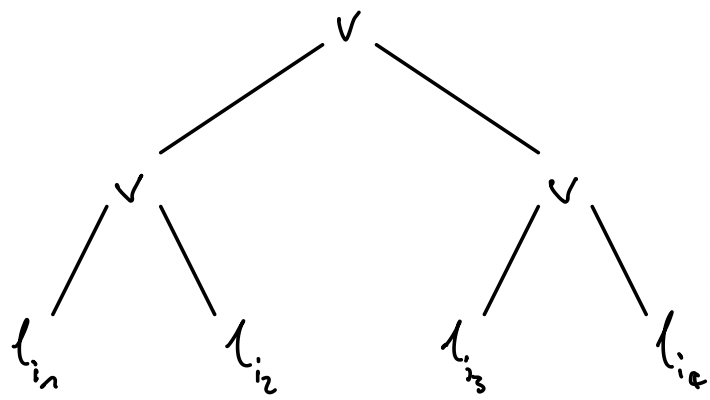
\includegraphics[width=.9\linewidth]{../assets/Screen Shot 2023-02-14 at 15.05.37.png}
\caption{\label{fig:org2b1a969}A syntax tree for clause \((l_{i_1}\vee l_{i_2}\vee l_{i_3}\vee l_{i_4})\)}
\end{figure}

For the root operator node, we introduce a \emph{clause vertex} \(u^i\) which is used by three flow pairs \(L,R,B\).
The idea is to guarantee that clause \(C_i\) is satisfied iff block \(b(u^i,L)\) is updated before block \(b(u^i,B)\) or block \(b(u^i,R)\) is updated before \(b(u^i,B)\).
Equivalently, \(b(u^i,B)\) cannot be updated unless at least one of \(b(u^i,L),b(u^i,R)\) has been updated.
Intuitively, if \(b(u^i,L)\) (\(b(u^i,R)\)) is updated before \(b(u^i,B)\), then the \(\textbf{L}\)eft half \((l_{i_1}\vee l_{i_2})\) (\(\textbf{R}\)ight half \((l_{i_3}\vee l_{i_4})\)) of \(C_i\) is satisfied.

Similarly, for the intermediate operator nodes of the syntax tree, we introduce clause vertices \(u_{1,2}^i,u_{3,4}^i\), where \(u_{1,2}^i\) corresponds to \((l_{i_1}\vee l_{i_2})\) and \(u_{3,4}^i\) corresponds to \((l_{i_3}\vee l_{i_4})\).
Both clause vertices are used by flow pairs \(\tilde{L},\tilde{R},\tilde{B}\) such that if \(b(u_{1,2}^i,\tilde{L})\) (\(b(u_{1,2}^i,\tilde{R})\)) is updated before \(b(u_{1,2},\tilde{B})\), then the left half \(l_{i_1}\) (right half \(l_{i_2}\)) of \((l_{i_1}\vee l_{i_2})\) is satisfied, and analogously for \(u_{3,4}^i\).

Moreover, for the operand nodes of the syntax tree, we introduce \emph{literal vertices} \(u_1^i,u_2^i,u_3^i,u_4^i\).

Finally, for every branch from a parent node to its left (right) child node, we add an edge to either \(L\) (\(R\)) (if the parent node is \(u^i\)) or \(\tilde{L}\) (\(\tilde{R}\)) (if the parent node is \(u_{1,2}^i\) or \(u_{3,4}^i\)).

We now proceed with the detailed specification of clause gadget \(C^i\) (see Figure \ref{fig:orgb090ce4}).

\begin{figure}[htbp]
\centering
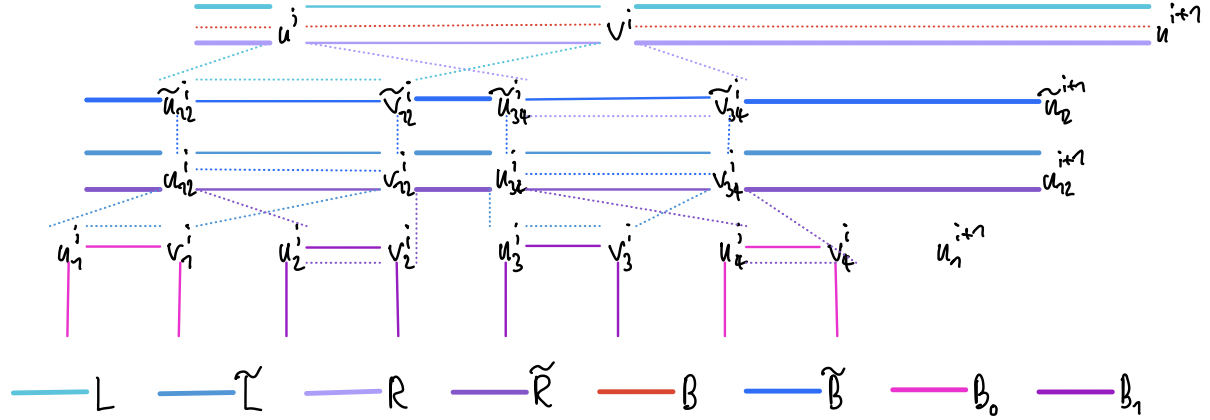
\includegraphics[width=.9\linewidth]{../assets/Screen Shot 2023-02-14 at 15.07.03.png}
\caption{\label{fig:orgb090ce4}Clause gadget \(C^i\)}
\end{figure}

We introduce six flow pairs \(L,R,B,\tilde{L},\tilde{R},\tilde{B}\), each with demand \(1\).

For the clause vertices, we introduce two vertices \(u^i,v^i\) and add edge \((u^i,v^i)\) to flows \(L^o,R^o,B^u\).
Similarly, we introduce vertices \(u_{1,2}^i,v_{1,2}^i,u_{3,4}^i,v_{3,4}^i\) and add edges \((u_{1,2}^i,v_{1,2}^i),(u_{3,4}^i,v_{3,4}^i)\) to flows \(\tilde{L}^o,\tilde{R}^o,\tilde{B}^u\).

For the literal vertices, we introduce vertices \(u_1^i,v_1^i,u_2^i,v_2^i,u_3^i,v_3^i,u_4^i,v_4^i\) and add edges \((u_1^i,v_1^i),(u_3^i,v_3^i)\) to flow \(\tilde{L}^u\) and \((u_2^i,v_2^i),(u_4^i,v_4^i)\) to \(\tilde{R}^u\).

Moreover, we introduce auxiliary vertices \(\tilde{u}_{1,2}^i,\tilde{v}_{1,2}^i,\tilde{u}_{3,4}^i,\tilde{v}_{3,4}^i\) and add edge \((\tilde{u}_{1,2}^i,\tilde{v}_{1,2}^i)\) to flows \(\tilde{L}^u,\tilde{B}^o\) and \((\tilde{u}_{3,4}^i,\tilde{v}_{3,4}^i)\) to \(\tilde{R}^u,\tilde{B}^o\).

Finally, we add the following edges to connect clause gadget \(C^i\):

\begin{itemize}
\item \((u^i,\tilde{u}_{1,2}^i),(\tilde{v}_{1,2}^i,v^i)\) to \(L^u\)
\item \((u^i,\tilde{u}_{3,4}^i),(\tilde{v}_{3,4}^i,v^i)\) to \(R^u\)
\item \((v_{1,2}^i,u_{3,4}^i)\) to \(\tilde{L}^o,\tilde{L}^u,\tilde{R}^o,\tilde{R}^u\)
\item \((u_{1,2}^i,u_1^i),(v_1^i,v_{1,2}^i),(u_{3,4}^i,u_3^i),(v_3^i,v_{3,4}^i)\) to \(\tilde{L}^u\)
\item \((u_{1,2}^i,u_2^i),(v_2^i,v_{1,2}^i),(u_{3,4}^i,u_4^i),(v_4^i,v_{3,4}^i)\) to \(\tilde{R}^u\)
\item \((\tilde{v}_{1,2}^i,\tilde{u}_{3,4}^i)\) to \(\tilde{B}^o,\tilde{B}^u\)
\item \((\tilde{u}_{1,2}^i,u_{1,2}^i),(v_{1,2}^i,\tilde{v}_{1,2}^i),(\tilde{u}_{3,4}^i,u_{3,4}^i),(v_{3,4}^i,\tilde{v}_{3,4}^i)\) to \(\tilde{B}^u\)
\end{itemize}

\paragraph{Variable gadgets.}
For every variable \(x_j\), we construct the corresponding variable gadget \(X^j\) as follows.
We introduce a \emph{variable vertex} \(x^j\) which is used by three flow pairs \(X,\bar{X},B\).
The idea is to guarantee the following:

\begin{enumerate}
\item If block \(b(x^j,X)\) is updated before block \(b(x^j,B)\), then variable \(x_j\) is assigned \(1\).
\item If block \(b(x^j,\bar{X})\) is updated before \(b(x^j,B)\), then \(x_j\) is assigned \(0\).
\item Not both \(b(x^j,X)\) and \(b(x^j,\bar{X})\) can be updated before \(b(x^j,B)\).
\end{enumerate}

We now proceed with the detailed specification of variable gadget \(X^j\) (see Figure \ref{fig:org28e35b2}).

\begin{figure}[htbp]
\centering
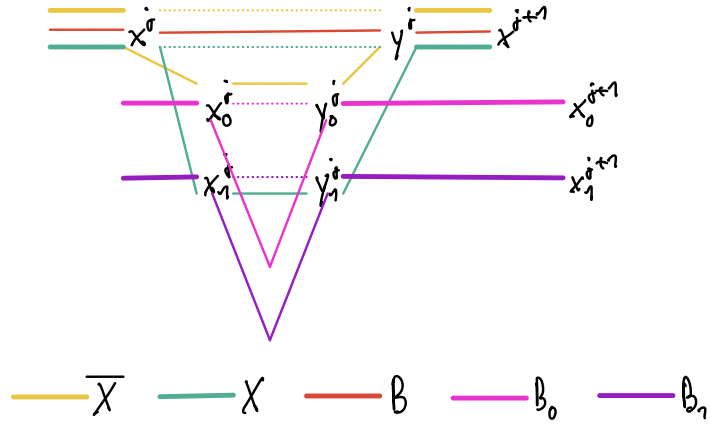
\includegraphics[width=.9\linewidth]{../assets/Screen Shot 2023-02-14 at 15.06.35.png}
\caption{\label{fig:org28e35b2}Variable gadget \(X^j\)}
\end{figure}

We introduce two flow pairs \(X,\bar{X}\), each with demand \(1\).
For the variable vertices, we introduce vertices \(x^j,y^j\) and add edge \((x^j,y^j)\) to flows \(X^u,\bar{X}^u,B^o\).
Moreover, we introduce auxiliary vertices \(x_0^j,y_0^j,x_1^j,y_1^j\) and add edge \((x_0^j,y_0^j)\) to flow \(\bar{X}^o\) and \((x_1^j,y_1^j)\) to \(X^o\).
Finally, to connect variable gadget \(X^j\), we add edges \((x^j,x_0^j),(y_0^j,y^j)\) to flow \(\bar{X}^o\) and \((x^j,x_1^j),(y_1^j,y^j)\) to \(X^o\).

\paragraph{Connecting variable with clause gadgets.}
For every \(j\in[n]\) and every \(i\in[m]\), we connect variable gadget \(X^j\) to clause gadget \(C^i\) if variable \(x_j\) occurs in clause \(C_i\).
More precisely, we introduce two flow pairs \(B_0,B_1\), each with demand \(1\), such that \(B_0\) (\(B_1\)) connects vertex \(x_0^j\) (\(x_1^j\)) to all literal vertices corresponding to literal \(\bar{x}_j\) (\(x_j\)).

More formally, for every \(j\in[n]\), let \(P_j=\{p_1^j,\dots,p_{\ell_j}^j\}\) denote the set of indices of the clauses containing literal \(x_j\) and \(\bar{P}_j=\{\bar{p}_1^j,\dots,p_{\ell'_j}^j\}\) denote the set of indices of the clauses containing literal \(\bar{x}_j\).
Moreover, for every \(j\in[n]\) and every \(i\in[m]\), let \(\pi(i,j)\) denote the position of literal \(x_j\) in clause \(C_i\) and \(\bar{\pi}(i,j)\) denote the position of literal \(\bar{x}_j\) in \(C_i\).
For every \(j\in[n]\), we add the following edges:

\begin{itemize}
\item \((x_0^j,u_{\bar{\pi}(\bar{p}_1^j,j)}^{\bar{p}_1^j})\), \((u_{\bar{\pi}(\bar{p}_{\ell}^j,j)}^{\bar{p}_{\ell}^j},v_{\bar{\pi}(\bar{p}_{\ell}^j,j)}^{\bar{p}_{\ell}^j})\) for every \(\ell\in[\ell'_j]\), \((v_{\bar{\pi}(\bar{p}_{\ell}^j,j)}^{\bar{p}_{\ell}^j},u_{\bar{\pi}(\bar{p}_{\ell+1}^j,j)}^{\bar{p}_{\ell+1}^j})\) for every \(\ell\in[\ell'_j-1]\), and \((v_{\bar{\pi}(\bar{p}_{\ell'_j}^j,j)}^{\bar{p}_{\ell'_j}^j},y_0^j)\) to \(B_0^o\)
\item \((x_1^j,u_{\pi(p_1^j,j)}^{p_1^j})\), \((u_{\pi(p_{\ell}^j,j)}^{p_{\ell}^j},v_{\pi(p_{\ell}^j,j)}^{p_{\ell}^j})\) for every \(\ell\in[\ell_j]\), \((v_{\pi(p_{\ell}^j,j)}^{p_{\ell}^j},u_{\pi(p_{\ell+1}^j,j)}^{p_{\ell+1}^j})\) for every \(\ell\in[\ell_j-1]\), and \((v_{\pi(p_{\ell_j}^j,j)}^{p_{\ell_j}^j},y_1^j)\) to \(B_1^o\)
\end{itemize}

\paragraph{Completing the update flow network.}
We introduce vertices \(s,t\) and create (\(s,t\))-paths for all flows by adding the following edges:

\begin{itemize}
\item \((s,u^1),(v^m,t)\) to \(L^o,L^u,R^o,R^u\)
\item \((v^i,u^{i+1})\) for every \(i\in[m-1]\) to \(L^o,L^u,R^o,R^u,B^u\)
\item \((s,u_{1,2}^1)\), \((v_{3,4}^i,u_{1,2}^{i+1})\) for every \(i\in[m-1]\), and \((v_{3,4}^m,t)\) to \(\tilde{L}^o,\tilde{L}^u,\tilde{R}^o,\tilde{R}^u\)
\item \((s,\tilde{u}_{1,2}^1)\), \((\tilde{v}_{3,4}^i,\tilde{u}_{1,2}^{i+1})\) for every \(i\in[m-1]\), and \((\tilde{v}_{3,4}^m,t)\) to \(\tilde{B}^o,\tilde{B}^u\)
\item \((s,x^1),(y^n,t)\) to \(X^o,X^u,\bar{X}^o,\bar{X}^u,B^o,B^u\)
\item \((y^j,x^{j+1})\) for every \(j\in[n-1]\) to \(X^o,X^u,\bar{X}^o,\bar{X}^u,B^o\)
\item \((x^1,u^1),(v^m,y^n)\) to \(B^u\)
\item \((s,x_0^1)\), \((y_0^j,x_0^{j+1})\) for every \(j\in[n-1]\), and \((y_0^n,t)\) to \(B_0^o,B_0^u\)
\item \((s,x_1^1)\), \((y_1^j,x_1^{j+1})\) for every \(j\in[n-1]\), and \((y_1^n,t)\) to \(B_1^o,B_1^u\)
\end{itemize}

See Figure \ref{fig:orgafeb507} for the complete update flow network and Table \ref{tab:orgd5acdff} for all (\(s,t\))-flows.

\begin{figure}[htbp]
\centering
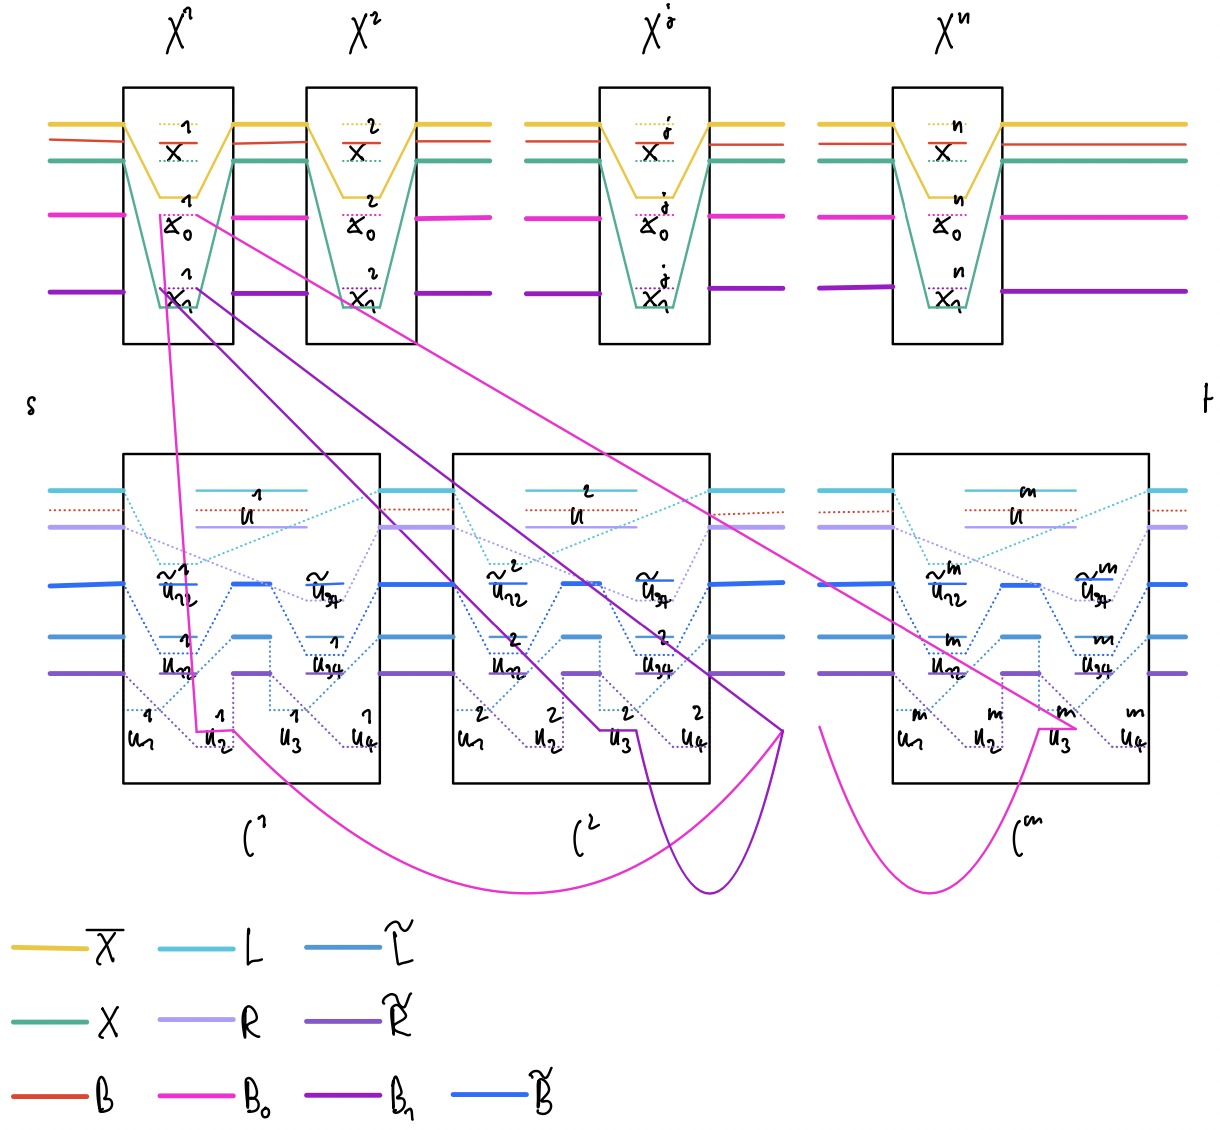
\includegraphics[width=.9\linewidth]{../assets/Screen Shot 2023-02-14 at 15.08.01.png}
\caption{\label{fig:orgafeb507}The update flow network}
\end{figure}

\begin{table}[htbp]
\caption{\label{tab:orgd5acdff}All (\(s,t\))-flows}
\centering
\begin{tabular}{ll}
Flow & (\(s,t\))-path\\[0pt]
\hline
\(\bar{X}^o\) & \(s,x^1,x_0^1,y_0^1,y^1,x^2,\dots,y^n,t\)\\[0pt]
\(\bar{X}^u\) & \(s,x^1,y^1,x^2,\dots,y^n,t\)\\[0pt]
\hline
\(L^o\) & \(s,u^1,v^1,u^2,\dots,v^m,t\)\\[0pt]
\(L^u\) & \(s,u^1,\tilde{u}_{1,2}^1,\tilde{v}_{1,2}^1,v^1,u^2,\dots,v^m,t\)\\[0pt]
\hline
\(\tilde{L}^o\) & \(s,u_{1,2}^1,v_{1,2}^1,u_{3,4}^1,v_{3,4}^1,u_{1,2}^2,\dots,v_{3,4}^m,t\)\\[0pt]
\(\tilde{L}^u\) & \(s,u_{1,2}^1,u_1^1,v_1^1,v_{1,2}^1,u_{3,4}^1,u_3^1,v_3^1,v_{3,4}^1,u_{1,2}^2,\dots,v_{3,4}^m,t\)\\[0pt]
\hline
\(X^o\) & \(s,x^1,x_1^1,y_1^1,y^1,x^2,\dots,y^n,t\)\\[0pt]
\(X^u\) & \(s,x^1,y^1,x^2,\dots,y^n,t\)\\[0pt]
\hline
\(R^o\) & \(s,u^1,v^1,u^2,\dots,v^m,t\)\\[0pt]
\(R^u\) & \(s,u^1,\tilde{u}_{3,4}^1,\tilde{v}_{3,4}^1,v^1,u^2,\dots,v^m,t\)\\[0pt]
\hline
\(\tilde{R}^o\) & \(s,u_{1,2}^1,v_{1,2}^1,u_{3,4}^1,v_{3,4}^1,u_{1,2}^2,\dots,v_{3,4}^m,t\)\\[0pt]
\(\tilde{R}^u\) & \(s,u_{1,2}^1,u_2^1,v_2^1,v_{1,2}^1,u_{3,4}^1,u_4^1,v_4^1,v_{3,4}^1,u_{1,2}^2,\dots,v_{3,4}^m,t\)\\[0pt]
\hline
\(B^o\) & \(s,x^1,y^1,x^2,\dots,y^n,t\)\\[0pt]
\(B^u\) & \(s,x^1,u^1,v^1,u^2,\dots,v^m,y^n,t\)\\[0pt]
\hline
\(\tilde{B}^o\) & \(s,\tilde{u}_{1,2}^1,\tilde{v}_{1,2}^1,\tilde{u}_{3,4}^1,\tilde{v}_{3,4}^1,\tilde{u}_{1,2}^2,\dots,\tilde{v}_{3,4}^m,t\)\\[0pt]
\(\tilde{B}^u\) & \(s,\tilde{u}_{1,2}^1,u_{1,2}^1,v_{1,2}^1,\tilde{v}_{1,2}^1,\tilde{u}_{3,4}^1,u_{3,4}^1,v_{3,4}^1,\tilde{v}_{3,4}^1,\tilde{u}_{1,2}^2,\dots,\tilde{v}_{3,4}^m,t^\)\\[0pt]
\hline
\(B_0^o\) & \(s,x_0^1,u_{\bar{\pi}(\bar{p}_1^1,1)}^{\bar{p}_1^1},v_{\bar{\pi}(\bar{p}_1^1,1)}^{\bar{p}_1^1},u_{\bar{\pi}(\bar{p}_2^1,1)}^{\bar{p}_2^1},\dots,v_{\bar{\pi}(\bar{p}_{l'_1}^1,1)}^{\bar{p}_{l'_1}^1},y_0^1,x_0^2,\dots,y_0^n,t\)\\[0pt]
\(B_0^u\) & \(s,x_0^1,y_0^1,x_0^2,\dots,y_0^n,t\)\\[0pt]
\hline
\(B_1^o\) & \(s,x_1^1,u_{\pi(p_1^1,1)}^{p_1^1},v_{\pi(p_1^1,1)}^{p_1^1},u_{\pi(p_2^1,1)}^{p_2^1},\dots,v_{\pi(p_{l_1}^1,1)}^{p_{l_1}^1},y_1^1,x_1^2,\dots,y_1^n,t\)\\[0pt]
\(B_1^u\) & \(s,x_1^1,y_1^1,x_1^2,\dots,y_1^n,t\)\\[0pt]
 & \\[0pt]
\end{tabular}
\end{table}

Edge capacities are defined as follows.

\begin{itemize}
\item We set the capacity to \(2\) for edges \((u^i,v^i),(u_{1,2}^i,v_{1,2}^i),(u_{3,4}^i,v_{3,4}^i),(x^j,y^j)\) for every \(i\in[m]\) and every \(j\in[n]\).
\item We set the capacity to \(1\) for edges \((u_1^i,v_1^i),(u_2^i,v_2^i),(u_3^i,v_3^i),(u_4^i,v_4^i),(\tilde{u}_{1,2}^i,\tilde{v}_{1,2}^i),(\tilde{u}_{3,4}^i,\tilde{v}_{3,4}^i),(x_0^j,y_0^j),(x_1^j,y_1^j)\) for every \(i\in[m]\) and every \(j\in[n]\).
\item All remaining edge capacities are set to \(10\), that is, the number of flow pairs, which equals the sum of all demands.
\end{itemize}

We remark that vertices \(\tilde{u}_{1,2}^i,\tilde{v}_{1,2}^i,\tilde{u}_{3,4}^i,\tilde{v}_{3,4}^i\) are not necessary for this proof.
Instead, we could directly connect clause vertices \(u^i,u_{1,2}^i\) via flow pair \(L\) and \(u^i,u_{3,4}^i\) via \(R\).
Similarly, vertices \(x_0^j,y_0^j,x_1^j,y_1^j\) as well as flow pairs \(B_0,B_1\) are not necessary.
We could instead directly connect variable vertex \(x^j\) to literal vertex, say \(u_1^i\), via \(X\) (\(\bar{X}\)) if \(l_{i_1}=x_j\) (\(l_{i_1}=\bar{x}_j\)).
The vertices and flow pairs are necessary, however, for the proof of Theorem \ref{org643d469}.

Let us quickly verify that \(G\) is a feasible update flow network.

To verify that every flow is indeed an \((s,t)\)-path, see Table \ref{tab:orgd5acdff}.
Recall we assumed every variable \(x_j\) occurs both negatively and positively in formula \(C\).
Hence both \(\bar{P}_j\) and \(P_j\) are non-empty.
Thus both \(B_0^o\) and \(B_1^o\) form \((s,t)\)-paths.

To verify that every flow pair forms a DAG, again consider Table \ref{tab:orgd5acdff}.

Using Lemma \ref{org51c1593}, we will show that all capacity constraints are satisfied for both the old flow network and the updated flow network in the if part of the proof of Theorem \ref{org3e793cd}.

\begin{table}[htbp]
\caption{\label{tab:orgd22e62f}All blocks grouped by flow pair}
\centering
\begin{tabular}{lll}
\(P\) & \(V(P^o\cap P^u)\) ordered w.r.t. \(\leq_{P^o\cup P^u}\) & \(B^P(G)\)\\[0pt]
\hline
\(\bar{X}\) & \(s,x^1,y^1,x^2,\dots,y^n,t\) & \(\{s,x^1\}\),\\[0pt]
 &  & \(\{x^j,x_0^j,y_0^j,y^j\},j\in[n]\),\\[0pt]
 &  & \(\{y^j,x^{j+1}\},j\in[n-1]\),\\[0pt]
 &  & \(\{y^n,t\}\)\\[0pt]
\hline
\(L\) & \(s,u^1,v^1,u^2,\dots,v^m,t\) & \(\{s,u^1\}\),\\[0pt]
 &  & \(\{u^i,\tilde{u}_{1,2}^i,\tilde{v}_{1,2}^i,v^i\},i\in[m]\),\\[0pt]
 &  & \(\{v^i,u^{i+1}\},i\in[m-1]\),\\[0pt]
 &  & \(\{v^m,t\}\)\\[0pt]
\hline
\(\tilde{L}\) & \(s,u_{1,2}^1,v_{1,2}^1,u_{3,4}^1,v_{3,4}^1,u_{1,2}^2,\dots,v_{3,4}^m,t\) & \(\{s,u_{1,2}^1\}\),\\[0pt]
 &  & \(\{u_{1,2}^i,u_1^i,v_1^i,v_{1,2}^i\},i\in[m]\),\\[0pt]
 &  & \(\{v_{1,2}^i,u_{3,4}^i\},i\in[m]\),\\[0pt]
 &  & \(\{u_{3,4}^i,u_3^i,v_3^i,v_{3,4}^i\},i\in[m]\),\\[0pt]
 &  & \(\{v_{3,4}^i,u_{1,2}^{i+1}\},i\in[m-1]\),\\[0pt]
 &  & \(\{v_{3,4}^m,t\}\)\\[0pt]
\hline
\(X\) & \(s,x^1,y^1,x^2,\dots,y^n,t\) & \(\{s,x^1\}\),\\[0pt]
 &  & \(\{x^j,x_1^j,y_1^j,y^j\},j\in[n]\),\\[0pt]
 &  & \(\{y^j,x^{j+1}\},j\in[n-1]\),\\[0pt]
 &  & \(\{y^n,t\}\)\\[0pt]
\hline
\(R\) & \(s,u^1,v^1,u^2,\dots,v^m,t\) & \(\{s,u^1\}\),\\[0pt]
 &  & \(\{u^i,\tilde{u}_{3,4}^i,\tilde{v}_{3,4}^i,v^i\},i\in[m]\),\\[0pt]
 &  & \(\{v^i,u^{i+1}\},i\in[m-1]\),\\[0pt]
 &  & \(\{v^m,t\}\)\\[0pt]
\hline
\(\tilde{R}\) & \(s,u_{1,2}^1,v_{1,2}^1,u_{3,4}^1,v_{3,4}^1,u_{1,2}^2,\dots,v_{3,4}^m,t\) & \(\{s,u_{1,2}^1\}\),\\[0pt]
 &  & \(\{u_{1,2}^i,u_2^i,v_2^i,v_{1,2}^i\},i\in[m]\),\\[0pt]
 &  & \(\{v_{1,2}^i,u_{3,4}^i\},i\in[m]\),\\[0pt]
 &  & \(\{u_{3,4}^i,u_4^i,v_4^i,v_{3,4}^i\},i\in[m]\),\\[0pt]
 &  & \(\{v_{3,4}^i,u_{1,2}^{i+1}\},i\in[m-1]\),\\[0pt]
 &  & \(\{v_{3,4}^m,t\}\)\\[0pt]
\hline
\(B\) & \(s,x^1,y^n,t\) & \(\{s,x^1\}\), \(\{x^j,y^j,u^i,v^i\mid j\in[n],i\in[m]\}\), \(\{y^n,t\}\)\\[0pt]
\hline
\(\tilde{B}\) & \(s,\tilde{u}_{1,2}^1,\tilde{v}_{1,2}^1,\tilde{u}_{3,4}^1,\tilde{v}_{3,4}^1,\tilde{u}_{1,2}^2,\dots,\tilde{v}_{3,4}^m,t\) & \(\{s,\tilde{u}_{1,2}^1\}\),\\[0pt]
 &  & \(\{\tilde{u}_{1,2}^i,u_{1,2}^i,v_{1,2}^i,\tilde{v}_{1,2}^i\},i\in[m]\),\\[0pt]
 &  & \(\{\tilde{v}_{1,2}^i,\tilde{u}_{3,4}^i\},i\in[m]\),\\[0pt]
 &  & \(\{\tilde{u}_{3,4}^i,u_{3,4}^i,v_{3,4}^i,\tilde{v}_{3,4}^i\},i\in[m]\),\\[0pt]
 &  & \(\{\tilde{v}_{3,4}^i,\tilde{u}_{1,2}^{i+1}\},i\in[m-1]\),\\[0pt]
 &  & \(\{\tilde{v}_{3,4}^m,t\}\)\\[0pt]
\hline
\(B_0\) & \(s,x_0^1,y_0^1,x_0^2,\dots,y_0^n,t\) & \(\{s,x_0^1\}\),\\[0pt]
 &  & \(\{x_0^j,u_{\bar{\pi}(i,j)}^i},v_{\bar{\pi}(i,j)}^i},y_0^j\mid i\in\bar{P}_j\},j\in[n]\),\\[0pt]
 &  & \(\{y_0^n,t\}\)\\[0pt]
\hline
\(B_1\) & \(s,x_1^1,y_1^1,x_1^2,\dots,y_1^n,t\) & \(\{s,x_1^1\}\),\\[0pt]
 &  & \(\{x_1^j,u_{\pi(i,j)}^i},v_{\pi(i,j)}^i},y_1^j\mid i\in P_j\},j\in[n]\),\\[0pt]
 &  & \(\{y_1^n,t\}\)\\[0pt]
 &  & \\[0pt]
\end{tabular}
\end{table}

\section{The Proof}
\label{sec:org50d40bd}

Before we prove Theorem \ref{org3e793cd}, let us show that every feasible block sequence for the update flow network specified in the previous section satisfies the following properties.

\begin{lem}
Let \(\mathcal{B}\) be a feasible block sequence for update flow network \(G\).
Then:

\begin{enumerate}
\item \label{itm:lem-feasible-block-sequence-properties-1}
For every \(i\in[m]\), \(\mathcal{B}(u^i,L)<\mathcal{B}(x^1,B)\) or \(\mathcal{B}(u^i,R)<\mathcal{B}(x^1,B)\).

\item \label{itm:lem-feasible-block-sequence-properties-2}
For every \(i\in[m]\),

\begin{enumerate}
\item \label{itm:lem-feasible-block-sequence-properties-2-1}
\(\mathcal{B}(\tilde{u}_{1,2}^i,\tilde{B})<\mathcal{B}(u^i,L)\), and

\item \label{itm:lem-feasible-block-sequence-properties-2-2}
\(\mathcal{B}(\tilde{u}_{3,4}^i,\tilde{B})<\mathcal{B}(u^i,R)\).
\end{enumerate}

\item \label{itm:lem-feasible-block-sequence-properties-3}
For every \(i\in[m]\),

\begin{enumerate}
\item \label{itm:lem-feasible-block-sequence-properties-3-1}
\(\mathcal{B}(u_{1,2}^i,\tilde{L})<\mathcal{B}(\tilde{u}_{1,2}^i,\tilde{B})\) or \(\mathcal{B}(u_{1,2}^i,\tilde{R})<\mathcal{B}(\tilde{u}_{1,2}^i,\tilde{B})\), and

\item \label{itm:lem-feasible-block-sequence-properties-3-2}
\(\mathcal{B}(u_{3,4}^i,\tilde{L})<\mathcal{B}(\tilde{u}_{3,4}^i,\tilde{B})\) or \(\mathcal{B}(u_{3,4}^i,\tilde{R})<\mathcal{B}(\tilde{u}_{3,4}^i,\tilde{B})\).
\end{enumerate}

\item \label{itm:lem-feasible-block-sequence-properties-4}
For every \(j\in[n]\), \(\mathcal{B}(x^1,B)<\mathcal{B}(x^j,\bar{X})\) or \(\mathcal{B}(x^1,B)<\mathcal{B}(x^j,X)\).

\item \label{itm:lem-feasible-block-sequence-properties-5}
For every \(i\in[m]\) and every \(j\in[n]\),

\begin{enumerate}
\item \label{itm:lem-feasible-block-sequence-properties-5-1}
if \(l_{i_1}=\bar{x}_j\), then \(\mathcal{B}(x_0^j,B_0)<\mathcal{B}(u_{1,2}^i,\tilde{L})\), and if \(l_{i_1}=x_j\), then \(\mathcal{B}(x_1^j,B_1)<\mathcal{B}(u_{1,2}^i,\tilde{L})\),

\item \label{itm:lem-feasible-block-sequence-properties-5-2}
if \(l_{i_2}=\bar{x}_j\), then \(\mathcal{B}(x_0^j,B_0)<\mathcal{B}(u_{1,2}^i,\tilde{R})\), and if \(l_{i_2}=x_j\), then \(\mathcal{B}(x_1^j,B_1)<\mathcal{B}(u_{1,2}^i,\tilde{R})\),

\item \label{itm:lem-feasible-block-sequence-properties-5-3}
if \(l_{i_3}=\bar{x}_j\), then \(\mathcal{B}(x_0^j,B_0)<\mathcal{B}(u_{3,4}^i,\tilde{L})\), and if \(l_{i_3}=x_j\), then \(\mathcal{B}(x_1^j,B_1)<\mathcal{B}(u_{3,4}^i,\tilde{L})\),

\item \label{itm:lem-feasible-block-sequence-properties-5-4}
if \(l_{i_4}=\bar{x}_j\), then \(\mathcal{B}(x_0^j,B_0)<\mathcal{B}(u_{3,4}^i,\tilde{R})\), and if \(l_{i_4}=x_j\), then \(\mathcal{B}(x_1^j,B_1)<\mathcal{B}(u_{3,4}^i,\tilde{R})\).
\end{enumerate}

\item \label{itm:lem-feasible-block-sequence-properties-6}
For every \(j\in[n]\),

\begin{enumerate}
\item \label{itm:lem-feasible-block-sequence-properties-6-1}
\(\mathcal{B}(x^j,\bar{X})<\mathcal{B}(x_0^j,B_0)\), and

\item \label{itm:lem-feasible-block-sequence-properties-6-2}
\(\mathcal{B}(x^j,X)<\mathcal{B}(x_1^j,B_1)\).
\end{enumerate}
\end{enumerate}
\label{org73aaf3e}
\end{lem}

\begin{proof}
We show every property by contradiction.
More precisely, for every property, we assume it doesn't hold and then obtain an edge and a round such that the corresponding capacity constraint is violated, which contradicts the feasibility of block sequence \(\mathcal{B}\).

Since every flow pair has demand \(1\), we may use \ref{orgd3eb958} to argue about capacity constraints.

\paragraph{\ref{itm:lem-feasible-block-sequence-properties-1}, \ref{itm:lem-feasible-block-sequence-properties-3}.}
We only show \ref{itm:lem-feasible-block-sequence-properties-1}; the proofs for \ref{itm:lem-feasible-block-sequence-properties-3-1} and \ref{itm:lem-feasible-block-sequence-properties-3-2} are analogous.
Suppose not.
Then obtain \(i\in[m]\) such that both \(\mathcal{B}(u^i,L)\geq\mathcal{B}(x^1,B)\) and \(\mathcal{B}(u^i,R)\geq\mathcal{B}(x^1,B)\).
We show that the capacity constraint for edge \((u^i,v^i)\) is violated for round \(\mathcal{B}(x^1,B)\).

We have that

\begin{enumerate}
\item \(\alpha_L((u^i,v^i),B_{\mathcal{B}(x^1,B)-1})=\mathrm{active}\), since \(b(u^i,L)\notin B_{\mathcal{B}(x^1,B)-1}\) and \((u^i,v^i)\in E(L^o)\),

\item \(\alpha_R((u^i,v^i),B_{\mathcal{B}(x^1,B)-1})=\mathrm{active}\), since \(b(u^i,R)\notin B_{\mathcal{B}(x^1,B)-1}\) and \((u^i,v^i)\in E(R^o)\), and

\item \(\alpha_B((u^i,v^i),B_{\mathcal{B}(x^1,B)})=\mathrm{active}\), since \(b(u^i,B)=b(x^1,B)\in B_{\mathcal{B}(x^1,B)}\) and \((u^i,v^i)\in E(B^u)\).
\end{enumerate}

Hence
\begin{align*}
\lvert\{P\in\mathcal{P}\mid&\alpha_P((u^i,v^i),B_{\mathcal{B}(x^1,B)-1})=\mathrm{active}\text{ or }\\
&\alpha_P((u^i,v^i),B_{\mathcal{B}(x^1,B)})=\mathrm{active}\}\rvert\geq\lvert\{L,R,B\}\rvert=3>2=c(u^i,v^i)
\end{align*}

\paragraph{\ref{itm:lem-feasible-block-sequence-properties-2}, \ref{itm:lem-feasible-block-sequence-properties-5}, \ref{itm:lem-feasible-block-sequence-properties-6}.}
We only show \ref{itm:lem-feasible-block-sequence-properties-2-1}; the proofs for \ref{itm:lem-feasible-block-sequence-properties-2-2}, \ref{itm:lem-feasible-block-sequence-properties-5-1}, \ref{itm:lem-feasible-block-sequence-properties-5-2}, \ref{itm:lem-feasible-block-sequence-properties-5-3}, \ref{itm:lem-feasible-block-sequence-properties-5-4}, \ref{itm:lem-feasible-block-sequence-properties-6-1}, and \ref{itm:lem-feasible-block-sequence-properties-6-2} are similar.
Suppose not.
Then obtain \(i\in[m]\) such that \(\mathcal{B}(\tilde{u}_{1,2}^i,\tilde{B})\geq\mathcal{B}(u^i,L)\).
We show that the capacity constraint for edge \((\tilde{u}_{1,2}^i,\tilde{v}_{1,2}^i)\) is violated for round \(\mathcal{B}(u^i,L)\).

We have that

\begin{enumerate}
\item \(\alpha_{\tilde{B}}((\tilde{u}_{1,2}^i,\tilde{v}_{1,2}^i),B_{\mathcal{B}(u^i,L)-1})=\mathrm{active}\), since \(b(\tilde{u}_{1,2}^i,\tilde{B})\notin B_{\mathcal{B}(u^i,L)-1}\) and \((\tilde{u}_{1,2}^i,\tilde{v}_{1,2}^i)\in E(\tilde{B}^o)\), and

\item \(\alpha_L((\tilde{u}_{1,2}^i,\tilde{v}_{1,2}^i),B_{\mathcal{B}(u^i,L)})=\mathrm{active}\), since \(b(\tilde{u}_{1,2}^i,L)=b(u^i,L)\in B_{\mathcal{B}(u^i,L)}\) and \((\tilde{u}_{1,2}^i,\tilde{v}_{1,2}^i)\in E(L^u)\).
\end{enumerate}

Hence
\begin{align*}
\lvert\{P\in\mathcal{P}\mid&\alpha_P((\tilde{u}_{1,2}^i,\tilde{v}_{1,2}^i),B_{\mathcal{B}(u^i,L)-1})=\mathrm{active}\text{ or }\\
&\alpha_P((\tilde{u}_{1,2}^i,\tilde{v}_{1,2}^i),B_{\mathcal{B}(u^i,L)})=\mathrm{active}\}\rvert\geq\lvert\{\tilde{B},L\}\rvert=2>1=c(\tilde{u}_{1,2}^i,\tilde{v}_{1,2}^i)
\end{align*}

\paragraph{\ref{itm:lem-feasible-block-sequence-properties-4}.}
Suppose not.
Then obtain \(j\in[n]\) such that both \(\mathcal{B}(x^1,B)\geq\mathcal{B}(x^j,\bar{X})\) and \(\mathcal{B}(x^1,B)\geq\mathcal{B}(x^j,X)\).
We show that the capacity constraint for edge \((x^j,y^j)\) is violated for round \(\mathcal{B}(x^1,B)\).

We have that

\begin{enumerate}
\item \(\alpha_B((x^j,y^j),B_{\mathcal{B}(x^1,B)-1})=\mathrm{active}\), since \(b(x^j,B)=b(x^1,B)\notin B_{\mathcal{B}(x^1,B)-1}\) and \((x^j,y^j)\in E(B^o)\),

\item \(\alpha_{\bar{X}}((x^j,y^j),B_{\mathcal{B}(x^1,B)})=\mathrm{active}\), since \(b(x^j,\bar{X})\notin B_{\mathcal{B}(x^1,B)}\) and \((x^j,y^j)\in E(\bar{X}^u)\), and

\item \(\alpha_{X}((x^j,y^j),B_{\mathcal{B}(x^1,B)})=\mathrm{active}\), since \(b(x^j,X)\notin B_{\mathcal{B}(x^1,B)}\) and \((x^j,y^j)\in E(X^u)\).
\end{enumerate}

Hence
\begin{align*}
\lvert\{P\in\mathcal{P}\mid&\alpha_P((x^j,y^j),B_{\mathcal{B}(x^1,B)-1})=\mathrm{active}\text{ or }\\
&\alpha_P((x^j,y^j),B_{\mathcal{B}(x^1,B)})=\mathrm{active}\}\rvert\geq\lvert\{B,\bar{X},X\}\rvert=3>2=c(x^j,y^j)
\end{align*}
\end{proof}

We are now ready to prove Theorem \ref{org3e793cd}.

\begin{proof}[Proof of Theorem [[thm:np-hardness-special-case]]]
We show that there is a satisfying assignment \(\sigma\) for 4CNF formula \(C\) iff there is a feasible block sequence \(\mathcal{B}\) for the corresponding update flow network \(G\), which, by Corollary \ref{org4ad2b7f}, is the case iff there is a feasible update sequence for \(G\).
We will choose \(\sigma\), \(\mathcal{B}\), respectively, such that \(\sigma\) assigns \(1\) to variable \(x_j\) iff \(\mathcal{B}(x^j,\bar{X})>\mathcal{B}(x^1,B)\).

\paragraph{Only-if part.}
Let \(\mathcal{B}\) be a feasible block sequence for \(G\).
We define assignment \(\sigma\) as follows:
For every variable \(x_j\), we assign \(1\) to \(x_j\) iff \(\mathcal{B}(x^j,\bar{X})>\mathcal{B}(x^1,B)\).
We now show that \(\sigma\) is a satisfying assignment for \(C\).

Let \(C_i=(l_{i_1}\vee l_{i_2}\vee l_{i_3}\vee l_{i_4})\) be a clause.
We show that \(\sigma\) satisfies \(C_i\) by obtaining a literal that evaluates to \(1\).

Consider round \(\mathcal{B}(x^1,B)\).
By Lemma \ref{org73aaf3e} \ref{itm:lem-feasible-block-sequence-properties-1}, \(\mathcal{B}(x^1,B)>\mathcal{B}(u^i,L)\) or \(\mathcal{B}(x^1,B)>\mathcal{B}(u^i,R)\).
We only consider the former case \(\mathcal{B}(x^1,B)>\mathcal{B}(u^i,L)\); the latter one is analogous.

By Lemma \ref{org73aaf3e} \ref{itm:lem-feasible-block-sequence-properties-2-1}, \(\mathcal{B}(u^i,L)>\mathcal{B}(\tilde{u}_{1,2}^i,\tilde{B})\).
By Lemma \ref{org73aaf3e} \ref{itm:lem-feasible-block-sequence-properties-3-1}, \(\mathcal{B}(\tilde{u}_{1,2}^i,\tilde{B})>\mathcal{B}(u_{1,2}^i,\tilde{L})\) or \(\mathcal{B}(\tilde{u}_{1,2}^i,\tilde{B})>\mathcal{B}(u_{1,2}^i,\tilde{R})\).
We only consider the latter case \(\mathcal{B}(\tilde{u}_{1,2}^i,\tilde{B})>\mathcal{B}(u_{1,2}^i,\tilde{R})\); the former one is analogous.

Let \(x_j\) be the variable corresponding to literal \(l_{i_2}\).
We consider the cases \(l_{i_2}=\bar{x}_j\) and \(l_{i_2}=x_j\) separately.

Case \(l_{i_2}=\bar{x}_j\).
By Lemma \ref{org73aaf3e} \ref{itm:lem-feasible-block-sequence-properties-5-2}, \(\mathcal{B}(u_{1,2}^i,\tilde{R})>\mathcal{B}(x_0^j,B_0)\).
By Lemma \ref{org73aaf3e} \ref{itm:lem-feasible-block-sequence-properties-6-1}, \(\mathcal{B}(x_0^j,B_0)>\mathcal{B}(x^j,\bar{X})\).
Putting everything together yields the following chain of inequalities:
\[
\mathcal{B}(x^1,B)>
\mathcal{B}(u^i,L)>
\mathcal{B}(\tilde{u}_{1,2}^i,\tilde{B})>
\mathcal{B}(u_{1,2}^i,\tilde{R})>
\mathcal{B}(x_0^j,B_0)>
\mathcal{B}(x^j,\bar{X})
\]
Hence, by definition of our assignment, variable \(x_j\) is assigned \(0\).
Hence literal \(l_{i_2}=\bar{x}_j\) evaluates to \(1\).

Case \(l_{i_2}=x_j\).
By Lemma \ref{org73aaf3e} \ref{itm:lem-feasible-block-sequence-properties-5-2}, \(\mathcal{B}(u_{1,2}^i,\tilde{R})>\mathcal{B}(x_1^j,B_1)\).
By Lemma \ref{org73aaf3e} \ref{itm:lem-feasible-block-sequence-properties-6-2}, \(\mathcal{B}(x_1^j,B_1)>\mathcal{B}(x^j,X)\).
Putting everything together yields the following chain of inequalities:
\[
\mathcal{B}(x^1,B)>
\mathcal{B}(u^i,L)>
\mathcal{B}(\tilde{u}_{1,2}^i,\tilde{B})>
\mathcal{B}(u_{1,2}^i,\tilde{R})>
\mathcal{B}(x_1^j,B_1)>
\mathcal{B}(x^j,X)
\]
Hence, by Lemma \ref{org73aaf3e} \ref{itm:lem-feasible-block-sequence-properties-4}, \(\mathcal{B}(x^j,\bar{X})>\mathcal{B}(x^1,B)\).
Hence, by definition of our assignment, variable \(x_j\) is assigned \(1\).
Hence literal \(l_{i_2}=x_j\) evaluates to \(1\).

\paragraph{If part.}
Let \(\sigma\) be a satisfying assignment for \(C\).
We construct a feasible block sequence \(\mathcal{B}=(\mathscr{B}_1,\dots,\mathscr{B}_{11})\) for \(G\) as follows.
The basic idea is to update blocks induced by

\begin{itemize}
\item variable vertices corresponding to variables that are assigned \(1\) and

\item clause vertices corresponding to satisfied clauses
\end{itemize}


before we update block \(b(x^1,B)\), and all other blocks afterwards.
We now specify \(\mathscr{B}_1,\dots,\mathscr{B}_{11}\) in detail.

\begin{enumerate}
\item For every variable \(x_j\), if \(x_j\) is assigned \(1\), we add block \(b(x^j,X)\) to \(\mathscr{B}_1\), otherwise we add \(b(x^j,\bar{X})\).
That is,
\[
   \mathscr{B}_1=\{b(x^j,X)\mid\sigma(x_j)=1\}\cup\{b(x^j,\bar{X}\mid\sigma(x_j)=0\}.
   \]

\item For every variable \(x_j\), if \(x_j\) is assigned \(1\), we add block \(b(x_1^j,B_1)\) to \(\mathscr{B}_2\), otherwise we add \(b(x_0^j,B_0)\).
That is,
\[
   \mathscr{B}_2=\{b(x_1^j,B_1)\mid\sigma(x_j)=1\}\cup\{b(x_0^j,B_0\mid\sigma(x_j)=0\}.
   \]

\item For every clause \(C_i=(l_{i_1}\vee l_{i_2}\vee l_{i_3}\vee l_{i_4})\),

\begin{enumerate}
\item if \(l_{i_1}\) evaluates to \(1\), we add block \(b(u_{1,2}^i,\tilde{L})\) to \(\mathscr{B}_3\),

\item if \(l_{i_2}\) evaluates to \(1\), we add \(b(u_{1,2}^i,\tilde{R})\),

\item if \(l_{i_3}\) evaluates to \(1\), we add \(b(u_{3,4}^i,\tilde{L})\), and

\item if \(l_{i_4}\) evaluates to \(1\), we add \(b(u_{3,4}^i,\tilde{R})\).
\end{enumerate}

That is,
\begin{align*}
\mathscr{B}_3=&\{b(u_{1,2}^i,\tilde{L})\mid\sigma(l_{i_1})=1\}\cup
\{b(u_{1,2}^i,\tilde{R})\mid\sigma(l_{i_2})=1\}\cup\\
&\{b(u_{3,4}^i,\tilde{L})\mid\sigma(l_{i_3})=1\}\cup
\{b(u_{3,4}^i,\tilde{R})\mid\sigma(l_{i_4})=1\}.
\end{align*}

\item For every clause \(C_i=(l_{i_1}\vee l_{i_2}\vee l_{i_3}\vee l_{i_4})\), if the left half \((l_{i_1}\vee l_{i_2})\) of \(C_i\) is satisfied, we add block \(b(\tilde{u}_{1,2}^i,\tilde{B})\) to \(\mathscr{B}_4\), and if the right half \((l_{i_3}\vee l_{i_4})\) is satisfied, we add \(b(\tilde{u}_{3,4}^i,\tilde{B})\).
That is,
\begin{align*}
\mathscr{B}_4=&\{b(\tilde{u}_{1,2}^i,\tilde{B})\mid\sigma(l_{i_1})=1\text{ or }\sigma(l_{i_2})=1\}\cup\\
&\{b(\tilde{u}_{3,4}^i,\tilde{B})\mid\sigma(l_{i_3})=1\text{ or }\sigma(l_{i_4})=1\}.
\end{align*}

\item For every clause \(C_i=(l_{i_1}\vee l_{i_2}\vee l_{i_3}\vee l_{i_4})\), if the left half \((l_{i_1}\vee l_{i_2})\) of \(C_i\) is satisfied, we add block \(b(u^i,L)\) to \(\mathscr{B}_5\), and if the right half \((l_{i_3}\vee l_{i_4})\) is satisfied, we add \(b(u^i,R)\).
That is,
\begin{align*}
\mathscr{B}_5=&\{b(u^i,L)\mid\sigma(l_{i_1})=1\text{ or }\sigma(l_{i_2})=1\}\cup\\
&\{b(u^i,R)\mid\sigma(l_{i_3})=1\text{ or }\sigma(l_{i_4})=1\}.
\end{align*}

\item \(\mathscr{B}_6=\{b(x^1,B)\}\).

\item For every variable \(x_j\), if \(x_j\) is assigned \(0\), we add block \(b(x^j,X)\) to \(\mathscr{B}_7\), otherwise we add \(b(x^j,\bar{X})\).
That is,
\[
   \mathscr{B}_7=\{b(x^j,X)\mid\sigma(x_j)=0\}\cup\{b(x^j,\bar{X}\mid\sigma(x_j)=1\}.
   \]

\item For every variable \(x_j\), if \(x_j\) is assigned \(0\), we add block \(b(x_1^j,B_1)\) to \(\mathscr{B}_8\), otherwise we add \(b(x_0^j,B_0)\).
That is,
\[
   \mathscr{B}_8=\{b(x_1^j,B_1)\mid\sigma(x_j)=0\}\cup\{b(x_0^j,B_0\mid\sigma(x_j)=1\}.
   \]

\item For every clause \(C_i=(l_{i_1}\vee l_{i_2}\vee l_{i_3}\vee l_{i_4})\),

\begin{enumerate}
\item if \(l_{i_1}\) evaluates to \(0\), we add block \(b(u_{1,2}^i,\tilde{L})\) to \(\mathscr{B}_9\),

\item if \(l_{i_2}\) evaluates to \(0\), we add \(b(u_{1,2}^i,\tilde{R})\),

\item if \(l_{i_3}\) evaluates to \(0\), we add \(b(u_{3,4}^i,\tilde{L})\), and

\item if \(l_{i_4}\) evaluates to \(0\), we add \(b(u_{3,4}^i,\tilde{R})\).
\end{enumerate}

That is,
\begin{align*}
\mathscr{B}_9=&\{b(u_{1,2}^i,\tilde{L})\mid\sigma(l_{i_1})=0\}\cup
\{b(u_{1,2}^i,\tilde{R})\mid\sigma(l_{i_2})=0\}\cup\\
&\{b(u_{3,4}^i,\tilde{L})\mid\sigma(l_{i_3})=0\}\cup
\{b(u_{3,4}^i,\tilde{R})\mid\sigma(l_{i_4})=0\}.
\end{align*}

\item For every clause \(C_i=(l_{i_1}\vee l_{i_2}\vee l_{i_3}\vee l_{i_4})\), if the left half \((l_{i_1}\vee l_{i_2})\) of \(C_i\) is unsatisfied, we add block \(b(\tilde{u}_{1,2}^i,\tilde{B})\) to \(\mathscr{B}_{10}\), and if the right half \((l_{i_3}\vee l_{i_4})\) is unsatisfied, we add \(b(\tilde{u}_{3,4}^i,\tilde{B})\).
That is,
\begin{align*}
\mathscr{B}_{10}=&\{b(\tilde{u}_{1,2}^i,\tilde{B})\mid\sigma(l_{i_1})=0\text{ and }\sigma(l_{i_2})=0\}\cup\\
&\{b(\tilde{u}_{3,4}^i,\tilde{B})\mid\sigma(l_{i_3})=0\text{ and }\sigma(l_{i_4})=0\}.
\end{align*}

\item For every clause \(C_i=(l_{i_1}\vee l_{i_2}\vee l_{i_3}\vee l_{i_4})\), if the left half \((l_{i_1}\vee l_{i_2})\) of \(C_i\) is unsatisfied, we add block \(b(u^i,L)\) to \(\mathscr{B}_{11}\), and if the right half \((l_{i_3}\vee l_{i_4})\) is unsatisfied, we add \(b(u^i,R)\).
That is,
\begin{align*}
\mathscr{B}_{11}=&\{b(u^i,L)\mid\sigma(l_{i_1})=0\text{ and }\sigma(l_{i_2})=0\}\cup\\
&\{b(u^i,R)\mid\sigma(l_{i_3})=0\text{ and }\sigma(l_{i_4})=0\}.
\end{align*}
\end{enumerate}

By Remark \ref{org22a2102}, we may ignore all other blocks.

We now show that block sequence \(\mathcal{B}=(\mathscr{B}_1,\dots,\mathscr{B}_{11})\) is feasible by verifying that the capacity constraint is satisfied for every edge and every \(\ell\in[11]\).
Since every flow pair has demand \(1\), we

\begin{itemize}
\item may use remark \ref{orgd3eb958} again to argue about capacity constraints, and

\item only have to consider edges with capacity less than \(10\), that is, the number of flow pairs.
\end{itemize}


For every such edge \(e\), we proceed as follows.

\begin{enumerate}
\item First, for every \(\ell\in\{0,\dots,11\}\) and every flow pair \(P\), we determine if \(e\) is on the transient (\(s,t\))-path for \(P\) after updating all blocks in \(B_{\ell}\), that is, we determine if \(\alpha_P(e,B_{\ell})=\mathrm{active}\).

\item Next, for every \(\ell\in\{0,\dots,11\}\), we determine the set of flow pairs \(P\) such that \(\alpha_P(e,B_{\ell})=\mathrm{active}\), that is, we determine the set \(\mathcal{P}(e,\ell):=\{P\in\mathcal{P}\mid\alpha_P(e,B_{\ell})=\mathrm{active}\}\).

\item Then, for every \(\ell\in[11]\), we determine the set \(\mathcal{P}'(e,\ell):=\mathcal{P}(e,\ell-1)\cup\mathcal{P}(e,\ell)=\{P\in\mathcal{P}\mid\alpha_P(e,B_{\ell-1})=\mathrm{active}\text{ or }\alpha_P(e,B_{\ell})=\mathrm{active}\}\).

\item Finally, for every \(\ell\in[11]\), we verify that the cardinality of the set \(\mathcal{P}'(e,\ell)\) obtained in the previous step is at most \(c(e)\).
\end{enumerate}


\paragraph{\((x^j,y^j)\)}
Let \(j\in[n]\).
Then edge \((x^j,y^j)\) is used by flow pairs \(\bar{X},X,B\).

Since \((x^j,y^j)\in E(\bar{X}^u\setminus\bar{X}^o)\), by Lemma \ref{org7e3e855},
\[\alpha_{\bar{X}}((x^j,y^j),B_{\ell})=
\begin{cases}
\mathrm{active} & \text{if }\sigma(x_j)=1\text{ and }\ell\geq 7\\
\mathrm{active} & \text{if }\sigma(x_j)=0\text{ and }\ell\geq 1\\
\mathrm{inactive} & \text{otherwise}.
\end{cases}\]

Since \((x^j,y^j)\in E(X^u\setminus X^o)\), by Lemma \ref{org7e3e855},
\[\alpha_X((x^j,y^j),B_{\ell})=
\begin{cases}
\mathrm{active} & \text{if }\sigma(x_j)=1\text{ and }\ell\geq 1\\
\mathrm{active} & \text{if }\sigma(x_j)=0\text{ and }\ell\geq 7\\
\mathrm{inactive} & \text{otherwise}.
\end{cases}\]

Since \((x^j,y^j)\in E(B^o\setminus B^u)\) and \(b(x^j,B)=b(x^1,B)\in\mathscr{B}_6\), by Lemma \ref{org7e3e855},
\[\alpha_B}((x^j,y^j),B_{\ell})=
\begin{cases}
\mathrm{active} & \ell<6\\
\mathrm{inactive} & \ell\geq 6.
\end{cases}\]

Hence,
\[\mathcal{P}((x^j,y^j),\ell)=
\begin{cases}
\{B\} & \ell<1\\
\{X,B\} & \sigma(x_j)=1\text{ and }1\leq\ell<6\\
\{X\} & \sigma(x_j)=1\text{ and }\ell=6\\
\{\bar{X},B\} & \sigma(x_j)=0\text{ and }1\leq\ell<6\\
\{\bar{X}\} & \sigma(x_j)=0\text{ and }\ell=6\\
\{\bar{X},X\} & \ell\geq 7.
\end{cases}\]

Hence,
\[\mathcal{P}'((x^j,y^j),\ell)=
\begin{cases}
\{X,B\} & \sigma(x_j)=1\text{ and }\ell<7\\
\{\bar{X},B\} & \sigma(x_j)=0\text{ and }\ell<7\\
\{\bar{X},X\} & \ell\geq 7.
\end{cases}\]

Hence \(\lvert\mathcal{P}'((x^j,y^j),\ell)\rvert=2=c(x^j,y^j)\) for every \(\ell\in[11]\).

\begin{itemize}
\item[{$\square$}] Repeat for other edges.
\end{itemize}
\end{proof}

\chapter{Merging Flow Pairs}
\label{sec:orgf460f2b}

We now prove the \hyperref[org1685041]{Merging Lemma}.

Let \(G=(V,E,\mathcal{P},s,t,c)\) be an update flow network with \(\lvert\mathcal{P}\rvert\geq 2\), and let \(F,F'\in\mathcal{P}\) and \(v_F,v_{F'}\in V\) such that they satisfy properties \ref{itm:lem-merging-flow-pairs-property-1}, \ref{itm:lem-merging-flow-pairs-property-2}, and \ref{itm:lem-merging-flow-pairs-property-3} (see Figure \ref{fig:org2d298b5}).
We construct an update flow network \(\tilde{G}=(\tilde{V},\tilde{E},\tilde{\mathcal{P}},s,t,\tilde{c})\) with \(\lvert\tilde{\mathcal{P}}\rvert=\lvert\mathcal{P}\rvert-1\) such that there is a feasible block sequence \(\mathcal{B}=(\mathscr{B}_1,\dots,\mathscr{B}_{\ell})\) for \(G\) iff there is a feasible block sequence \(\tilde{\mathcal{B}}=(\tilde{\mathscr{B}}_1,\dots,\tilde{\mathscr{B}}_{\ell})\) for \(\tilde{G}\) as follows.

\begin{figure}[htbp]
\centering
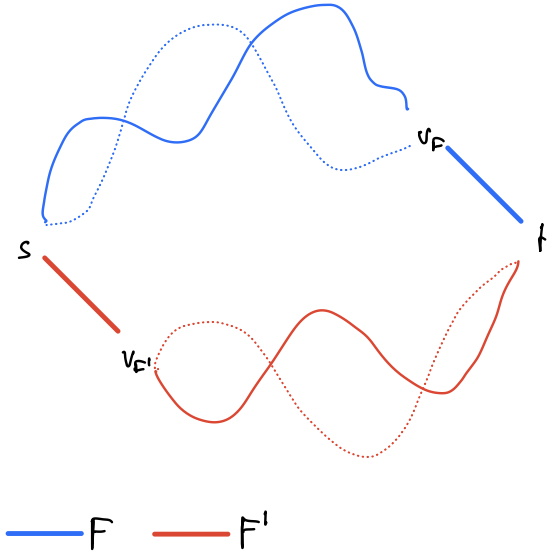
\includegraphics[width=.9\linewidth]{../assets/Screen Shot 2023-02-19 at 13.28.41.png}
\caption{\label{fig:org2d298b5}Flow pairs \(F\) and \(F'\) in update flow network \(G\)}
\end{figure}

\section{The Construction}
\label{sec:orgf6c07f7}

Intuitively, we merge flow pairs \(F\) and \(F'\) into a single flow pair \(\tilde{F}\) by concatenating \(F\) and \(F'\).
More precisely, \(\tilde{F}\) will be the union of \(F\) and \(F'\) except that we replace edges \((v_F,t)\) and \((s,v_{F'})\) by edge \((v_F,v_{F'})\) (see Figure \ref{fig:orgb99869b} for an illustration).
More formally, we define flow pair \(\tilde{F}\) as follows:

\begin{align*}
\tilde{E}(\tilde{F}^o)&=\left(E(F^o)\setminus\{(v_F,t)\}\right)\cup\left(E(F'^o)\setminus\{(s,v_{F'})\}\right)\cup\{(v_F,v_{F'})\}\\
\tilde{E}(\tilde{F}^u)&=\left(E(F^u)\setminus\{(v_F,t)\}\right)\cup\left(E(F'^u)\setminus\{(s,v_{F'})\}\right)\cup\{(v_F,v_{F'})\}\\
\tilde{V}(\tilde{F}^o)&=\tilde{V}(\tilde{E}(\tilde{F}^o))\\
\tilde{V}(\tilde{F}^u)&=\tilde{V}(\tilde{E}(\tilde{F}^u))\\
\tilde{d}_{\tilde{F}}&=d_F
\end{align*}

\begin{figure}[htbp]
\centering
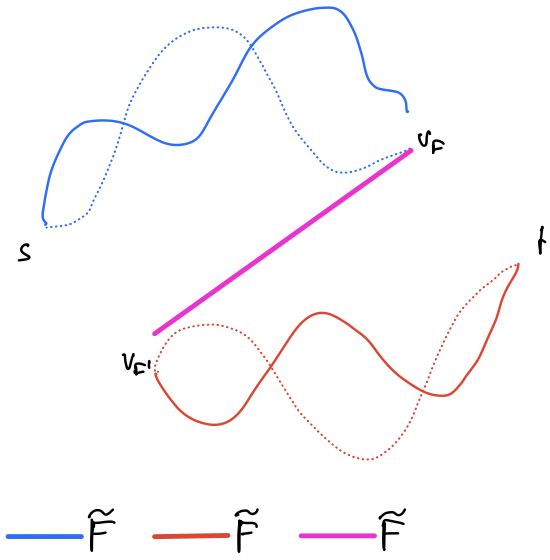
\includegraphics[width=.9\linewidth]{../assets/Screen Shot 2023-02-19 at 13.29.07.png}
\caption{\label{fig:orgb99869b}Flow pair \(\tilde{F}\) in update flow network \(\tilde{G}\)}
\end{figure}

Update flow network \(\tilde{G}=(\tilde{V},\tilde{E},\tilde{\mathcal{P}},s,t,\tilde{c})\) is defined as follows:

\begin{align*}
\tilde{\mathcal{P}}&=\mathcal{P}\setminus\{F,F'\}\cup\{\tilde{F}\}\\
\tilde{V}&=\bigcup_{\tilde{P}\in\tilde{\mathcal{P}}}\tilde{V}(\tilde{P}^o\cup\tilde{P}^u)\\
\tilde{E}&=\bigcup_{\tilde{P}\in\tilde{\mathcal{P}}}\tilde{E}(\tilde{P}^o\cup\tilde{P}^u)\\
\tilde{c}(\tilde{e})&=
\begin{cases}
\sum_{\tilde{P}\in\tilde{\mathcal{P}}:\tilde{e}\in\tilde{E}(\tilde{P}^o\cup\tilde{P}^u)}\tilde{d}_{\tilde{P}} & \text{if }\tilde{e}=(v_F,v_{F'})\\
c(\tilde{e}) & \text{otherwise}
\end{cases}
\end{align*}

Let us quickly verify that \(\tilde{G}\) is a feasible update flow network.

Let \(\tilde{P}\in\tilde{\mathcal{P}}\).
If \(\tilde{P}\neq\tilde{F}\), then \(\tilde{P}\in\mathcal{P}\) and hence, by feasibility of update flow network \(G\), both \(\tilde{P}^o\) and \(\tilde{P}^u\) are \((s,t)\)-paths in \(\tilde{G}\) and \(\tilde{P}\) forms a DAG.
Now suppose \(\tilde{P}=\tilde{F}\).
By feasibility of \(G\) and construction of \(\tilde{F}\), \(\tilde{F}^o\) (\(\tilde{F}^u\)) comprises the \((s,v_F)\)-path in \(F^o\) (\(F^u\)), edge \((v_F,v_{F'})\), and the \((v_{F'},t)\)-path in \(F'^o\) (\(F'^u\)), and hence forms an \((s,t)\)-path.
Moreover, since, again by feasibility of \(G\), both \(F\) and \(F'\) form DAGs, and edge \((v_F,v_{F'})\) does not introduce a cycle, as \(F\) and \(F'\) have no common vertices other than \(s,t\) by assumption, \(\tilde{F}\) forms a DAG.

Using Lemma \ref{org51c1593}, we will show that all capacity constraits are satisfied for both the old flow network and the updated flow network in the if part of the proof of the \hyperref[org1685041]{Merging Lemma}.

We denote notations such as \(b(v,P)\), \(B_i\), and \(\alpha_P(e,B)\) referring to update flow network \(\tilde{G}\) by \(\tilde{b}(v,P)\), \(\tilde{B}_i\), and \(\tilde{\alpha}_P(e,B)\).

\section{The Proof}
\label{sec:org88de7a0}

Our goal is to show that there is a feasible block sequence \(\mathcal{B}=(\mathscr{B}_1,\dots,\mathscr{B}_{\ell})\) for \(G\) iff there is a feasible block sequence \(\tilde{\mathcal{B}}=(\tilde{\mathscr{B}}_1,\dots,\tilde{\mathscr{B}}_{\ell})\) for \(\tilde{G}\).
We will choose \(\mathcal{B},\tilde{\mathcal{B}}\), respectively, such that, for every block \(b\) contained in both \(G\) and \(\tilde{G}\), \(b\) is updated in round \(i\in[\ell]\) in \(\mathcal{B}\) iff it is updated in round \(i\) in \(\tilde{\mathcal{B}}\), that is, \(\mathcal{B}(b)=\tilde{\mathcal{B}}(b)\).
The key insight is that it is indeed sufficient to consider such blocks.

\begin{lem}
~
\begin{enumerate}
\item \label{itm:lem-p-blocks-1}
Let \(\tilde{u}\in\tilde{V}(\tilde{F}^o\cup\tilde{F}^u)\setminus\{v_F\}\). Then:

\begin{enumerate}
\item \label{itm:lem-p-blocks-1-1}
If \(\tilde{u}\in V(F^o\cup F^u)\), then \(\tilde{b}(\tilde{u},\tilde{F})=b(\tilde{u},F)\).

\item \label{itm:lem-p-blocks-1-2}
If \(\tilde{u}\in V(F'^o\cup F'^u)\setminus\{s\}\), then \(\tilde{b}(\tilde{u},\tilde{F})=b(\tilde{u},F')\).
\end{enumerate}

\item \label{itm:lem-p-blocks-2}
For every \(\tilde{P}\in\tilde{\mathcal{P}}\setminus\{\tilde{F}\}\) and every \(\tilde{u}\in\tilde{V}(\tilde{P}^o\cup\tilde{P}^u)\), \(\tilde{b}(\tilde{u},\tilde{P})=b(\tilde{u},\tilde{P})\).
\end{enumerate}
\label{org6d87070}
\end{lem}

\begin{remark}
The proof is very technical and tedious--and hence omitted for now--and I hope we can come up with a better characterization of blocks (see \url{../README.org}) which significantly simplifies the proof.
\end{remark}

\begin{corollary}
~
\begin{enumerate}
\item \label{itm:corollary-p-blocks-1}
For every block \(\tilde{b}\in\tilde{B}(\tilde{G})\setminus\{\{v_F,v_{F'}\}\}\), \(\tilde{b}\in B(G)\).

\item \label{itm:corollary-p-blocks-2}
For every block \(b\in B(G)\setminus\{\{v_F,t\},\{s,v_{F'}\}\}\), \(b\in\tilde{B}(\tilde{G})\).
\end{enumerate}
\label{orgd07a2c6}
\end{corollary}

\begin{proof}
~
\paragraph{\ref{itm:corollary-p-blocks-1}.}
Let \(\tilde{b}\in\tilde{B}(\tilde{G})\setminus\{\{v_F,v_{F'}\}\}\), \(\tilde{P}=\tilde{P}(\tilde{b})\), and \(\tilde{u}=\tilde{\mathcal{S}}(\tilde{b})\).
If \(\tilde{P}=\tilde{F}\), then, by assumption, \(\tilde{u}\neq v_F\) and hence, by construction of \(\tilde{F}\) and Lemma \ref{org6d87070} \ref{itm:lem-p-blocks-1}, \(\tilde{b}=b(\tilde{u},F)\in B(G)\) or \(\tilde{b}=b(\tilde{u},F')\in B(G)\).
If \(\tilde{P}\neq\tilde{F}\), then, by Lemma \ref{org6d87070} \ref{itm:lem-p-blocks-2}, \(\tilde{b}=b(\tilde{u},\tilde{P})\in B(G)\).


\paragraph{\ref{itm:corollary-p-blocks-2}.}
Let \(b\in B(G)\setminus\{\{v_F,t\},\{s,v_{F'}\}\}\), \(P=P(b)\), and \(u=\mathcal{S}(b)\).
If \(P=F\), then, by assumption, \(u\neq v_F\) and hence, by construction of \(\tilde{F}\) and Lemma \ref{org6d87070} \ref{itm:lem-p-blocks-1-1}, \(b=\tilde{b}(u,\tilde{F})\in\tilde{B}(\tilde{G})\).
If \(P=F'\), then, by assumption, \(u\notin\{v_F,s\}\) and hence, by construction of \(\tilde{F}\) and Lemma \ref{org6d87070} \ref{itm:lem-p-blocks-1-2}, \(b=\tilde{b}(u,\tilde{F})\in\tilde{B}(\tilde{G})\).
If \(P\in\mathcal{P}\setminus\{F,F'\}\), then \(P\in\tilde{\mathcal{P}}\setminus\{\tilde{F}\}\) and hence, by Lemma \ref{org6d87070} \ref{itm:lem-p-blocks-2}, \(b=\tilde{b}(u,P)\in\tilde{B}(\tilde{G})\).
\end{proof}

To show that block sequences \(\mathcal{B},\tilde{\mathcal{B}}\) as chosen above are feasible, we will verify that capacity constraint \ref{eq:orgaadab49} is satisfied for every edge \(e\in E\), \(\tilde{e}\in\tilde{E}\), respectively, and every \(i\in[\ell]\).
We now show that for every edge \(\tilde{e}\) other than \((v_F,t),(s,v_{F'}),(v_F,v_{F'})\) and every \(i\in[\ell]\), \(\tilde{e}\) is on some transient (\(s,t\))-path in \(\tilde{G}\) after updating all blocks in \(\tilde{B}_i\) iff it is on some transient (\(s,t\))-path in \(G\) after updating all blocks in \(B_i\).

\begin{lem}
Let \(\mathcal{B}=(\mathscr{B}_1,\dots,\mathscr{B}_{\ell})\) be a block sequence for \(G\) and \(\tilde{\mathcal{B}}=(\tilde{\mathscr{B}}_1,\dots,\tilde{\mathscr{B}}_{\ell})\) be a block sequence for \(\tilde{G}\) such that for every block \(b\) contained in both \(G\) and \(\tilde{G}\), \(\mathcal{B}(b)=\tilde{\mathcal{B}}(b)\).
Moreover, let \((\tilde{u},\tilde{v})\in\tilde{E}\setminus\{(v_F,t),(s,v_{F'}),(v_F,v_{F'})\}\) and \(i\in[\ell]\).
Finally, let \(\tilde{P}\in\tilde{\mathcal{P}}\) such that \((\tilde{u},\tilde{v})\in\tilde{E}(\tilde{P}^o\cup\tilde{P}^u)\).
Then:

\begin{enumerate}
\item \label{itm:lem-alpha-1}
If \(\tilde{P}=\tilde{F}\), then \(\tilde{\alpha}_{\tilde{P}}((\tilde{u},\tilde{v}),\tilde{B}_i)=\mathrm{active}\) iff either \(\alpha_F((\tilde{u},\tilde{v}),B_i)=\mathrm{active}\) or \(\alpha_{F'}((\tilde{u},\tilde{v}),B_i)=\mathrm{active}\).

\item \label{itm:lem-alpha-2}
If \(\tilde{P}\neq\tilde{F}\), then \(\tilde{\alpha}_{\tilde{P}}((\tilde{u},\tilde{v}),\tilde{B}_i)=\alpha_{\tilde{P}}((\tilde{u},\tilde{v}),B_i)\).
\end{enumerate}
\label{org35f31be}
\end{lem}

\begin{proof}
Let \(\mathcal{B}=(\mathscr{B}_1,\dots,\mathscr{B}_{\ell})\) be a block sequence for \(G\) and \(\tilde{\mathcal{B}}=(\tilde{\mathscr{B}}_1,\dots,\tilde{\mathscr{B}}_{\ell})\) be a block sequence for \(\tilde{G}\) such that for every block \(b\) satisfying both \(b\in B(G)\) and \(b\in\tilde{B}(\tilde{G})\), \(\mathcal{B}(b)=\tilde{\mathcal{B}}(b)\).
Let \((\tilde{u},\tilde{v})\in\tilde{E}\setminus\{(v_F,t),(s,v_{F'}),(v_F,v_{F'})\}\) and \(i\in[\ell]\).
Let \(\tilde{P}\in\tilde{\mathcal{P}}\) such that \((\tilde{u},\tilde{v})\in\tilde{E}(\tilde{P}^o\cup\tilde{P}^u)\).

\paragraph{\ref{itm:lem-alpha-1}.}
Suppose \(\tilde{P}=\tilde{F}\).
By definition of \(\tilde{F}\) and since \((\tilde{u},\tilde{v})\in\tilde{E}\setminus\{(v_F,t),(s,v_{F'}),(v_F,v_{F'})\}\), \((\tilde{u},\tilde{v})\in\tilde{E}(\tilde{F}^o)\) iff \((\tilde{u},\tilde{v})\in E(F^o)\) or \((\tilde{u},\tilde{v})\in E(F'^o)\).
Similarly, \((\tilde{u},\tilde{v})\in\tilde{E}(\tilde{F}^u)\) iff \((\tilde{u},\tilde{v})\in E(F^u)\) or \((\tilde{u},\tilde{v})\in E(F'^u)\).
We show \(\tilde{\alpha}_{\tilde{F}}((\tilde{u},\tilde{v}),\tilde{B}_i)=\mathrm{active}\) iff \(\alpha_F((\tilde{u},\tilde{v}),B_i)=\mathrm{active}\) or \(\alpha_{F'}((\tilde{u},\tilde{v}),B_i)=\mathrm{active}\).
Notice that this implies \ref{itm:lem-alpha-1}, since, by assumption, \(F,F'\) are edge-disjoint: Otherwise, either

\begin{enumerate}
\item \(F\) and \(F'\) have a common vertex other than \(s,t\), or

\item \(F^o\cup F^u\) and \(F'^o\cup F'^u\) both consist of the single edge \((s,t)\), in which case \(v_F=s\) and \(v_{F'}=t\), which contradicts that \((v_F,v_{F'})\notin E\).
\end{enumerate}


We first show the if part.
Suppose \(\tilde{\alpha}_{\tilde{F}}((\tilde{u},\tilde{v}),\tilde{B}_i)=\mathrm{active}\).
By assumption, \((\tilde{u},\tilde{v})\in\tilde{E}(\tilde{F}^o)\) or \((\tilde{u},\tilde{v})\in\tilde{E}(\tilde{F}^u)\).
Hence \((\tilde{u},\tilde{v})\in E(F^o)\) or \((\tilde{u},\tilde{v})\in E(F^u)\) or \((\tilde{u},\tilde{v})\in E(F'^o)\) or \((\tilde{u},\tilde{v})\in E(F'^u)\).
We only consider case \((\tilde{u},\tilde{v})\in E(F^o)\); case \((\tilde{u},\tilde{v})\in E(F^u)\) is similar, and cases \((\tilde{u},\tilde{v})\in E(F'^o)\), \((\tilde{u},\tilde{v})\in E(F'^u)\) are analogous to cases \((\tilde{u},\tilde{v})\in E(F^o)\), \((\tilde{u},\tilde{v})\in E(F^u)\), respectively.

Suppose \((\tilde{u},\tilde{v})\in E(F^o)\).
Hence \((\tilde{u},\tilde{v})\in\tilde{E}(\tilde{F}^o)\).
Hence \(\tilde{b}(\tilde{u},\tilde{F})\in\tilde{B}_i\).
Moreover, by Lemma \ref{org6d87070} \ref{itm:lem-p-blocks-1-1}, \(\tilde{b}(\tilde{u},\tilde{F})=b(\tilde{u},F)\).
Hence, by assumption, \(b(\tilde{u},F)\in B_i\).
Thus \(\alpha_F((\tilde{u},\tilde{v}),B_i)=\mathrm{active}\).

We now show the only-if part.
Suppose \(\alpha_F((\tilde{u},\tilde{v}),B_i)=\mathrm{active}\) or \(\alpha_{F'}((\tilde{u},\tilde{v}),B_i)=\mathrm{active}\).
We only consider the former case; the latter one is analogous.

Suppose \(\alpha_F((\tilde{u},\tilde{v}),B_i)=\mathrm{active}\).
Hence \((\tilde{u},\tilde{v})\in E(F^o)\) or \((\tilde{u},\tilde{v})\in E(F^u)\).
We again only consider the former case; the latter one is similar.

Suppose \((\tilde{u},\tilde{v})\in E(F^o)\).
Hence \(b(\tilde{u},F)\in B_i\).
Moreover, by Lemma \ref{org6d87070} \ref{itm:lem-p-blocks-1-1}, \(b(\tilde{u},F)=\tilde{b}(\tilde{u},\tilde{F})\).
Hence, by assumption, \(\tilde{b}(\tilde{u},\tilde{F})\in\tilde{B}_i\).
Moreover, \((\tilde{u},\tilde{v})\in\tilde{E}(\tilde{F}^o)\).
Thus \(\tilde{\alpha}_{\tilde{F}}((\tilde{u},\tilde{v}),\tilde{B}_i)=\mathrm{active}\).

\paragraph{\ref{itm:lem-alpha-2}.}
Suppose \(\tilde{P}\neq\tilde{F}\).
By definition of \(\tilde{G}\), \(\tilde{P}\in\mathcal{P}\setminus\{F,F'\}\) and hence both \((\tilde{u},\tilde{v})\in\tilde{E}(\tilde{P}^o)\) iff \((\tilde{u},\tilde{v})\in E(\tilde{P}^o)\) and \((\tilde{u},\tilde{v})\in\tilde{E}(\tilde{P}^u)\) iff \((\tilde{u},\tilde{v})\in E(\tilde{P}^u)\).
Hence \(\tilde{b}(\tilde{u},\tilde{P})\in\tilde{B}(\tilde{G})\) and \(\tilde{b}(\tilde{u},\tilde{P})\in B(G)\).
Hence, by assumption, \(\tilde{b}(\tilde{u},\tilde{P})\in\tilde{B}_i\) iff \(\tilde{b}(\tilde{u},\tilde{P})\in B_i\), and, by Lemma \ref{org6d87070} \ref{itm:lem-p-blocks-2}, \(\tilde{b}(\tilde{u},\tilde{P})=b(\tilde{u},\tilde{P})\).
Hence \(\tilde{b}(\tilde{u},\tilde{P})\in\tilde{B}_i\) iff \(b(\tilde{u},\tilde{P})\in B_i\).
The claim now follows by definitions of \(\tilde{\alpha}_{\tilde{P}},\alpha_{\tilde{P}}\).
\end{proof}

\begin{lem}
Let \(\mathcal{B}=(\mathscr{B}_1,\dots,\mathscr{B}_{\ell})\) be a block sequence for \(G\) and \(\tilde{\mathcal{B}}=(\tilde{\mathscr{B}}_1,\dots,\tilde{\mathscr{B}}_{\ell})\) be a block sequence for \(\tilde{G}\) such that for every block \(b\) contained in both \(G\) and \(\tilde{G}\), \(\mathcal{B}(b)=\tilde{\mathcal{B}}(b)\).
Moreover, let \((\tilde{u},\tilde{v})\in\tilde{E}\setminus\{(v_F,t),(s,v_{F'}),(v_F,v_{F'})\}\) and \(i\in[\ell]\).
Then

\begin{align*}
\sum_{\tilde{P}\in\tilde{\mathcal{P}}:\tilde{\alpha}_{\tilde{P}}((\tilde{u},\tilde{v}),\tilde{B}_{i-1})=\mathrm{active}\text{ or }\tilde{\alpha}_{\tilde{P}}((\tilde{u},\tilde{v}),\tilde{B}_i)=\mathrm{active}}\tilde{d}_{\tilde{P}}&=\\
\sum_{\tilde{P}\in\mathcal{P}:\alpha_{\tilde{P}}((\tilde{u},\tilde{v}),B_{i-1})=\mathrm{active}\text{ or }\alpha_{\tilde{P}}((\tilde{u},\tilde{v}),B_i)=\mathrm{active}}d_{\tilde{P}}&.
\end{align*}
\label{org8a5fb8c}
\end{lem}

\begin{proof}
Let \(\mathcal{B}=(\mathscr{B}_1,\dots,\mathscr{B}_{\ell})\) be a block sequence for \(G\) and \(\tilde{\mathcal{B}}=(\tilde{\mathscr{B}}_1,\dots,\tilde{\mathscr{B}}_{\ell})\) be a block sequence for \(\tilde{G}\) such that for every block \(b\) satisfying both \(b\in B(G)\) and \(b\in\tilde{B}(\tilde{G})\), \(\mathcal{B}(b)=\tilde{\mathcal{B}}(b)\).
Let \((\tilde{u},\tilde{v})\in\tilde{E}\setminus\{(v_F,t),(s,v_{F'}),(v_F,v_{F'})\}\) and \(i\in[\ell]\).
By definition of \(\tilde{G}\), \(\tilde{\mathcal{P}}=\mathcal{P}\setminus\{F,F'\}\cup\{\tilde{F}\}\), \(\tilde{d}_{\tilde{F}}=d_F\), and \(\tilde{d}_{\tilde{P}}=d_{\tilde{P}}\) for every \(\tilde{P}\in\tilde{\mathcal{P}}\setminus\{\tilde{F}\}\).
Moreover, by assumption, \(d_F=d_{F'}\).
Hence, by Lemma \ref{org35f31be}, we have

\begin{align*}
\sum_{\tilde{P}\in\tilde{\mathcal{P}}:\tilde{\alpha}_{\tilde{P}}((\tilde{u},\tilde{v}),\tilde{B}_{i-1})=\mathrm{active}\text{ or }\tilde{\alpha}_{\tilde{P}}((\tilde{u},\tilde{v}),\tilde{B}_i)=\mathrm{active}}\tilde{d}_{\tilde{P}}&=\\
\sum_{\tilde{P}\in\tilde{\mathcal{P}}\setminus\{\tilde{F}\}:\tilde{\alpha}_{\tilde{P}}((\tilde{u},\tilde{v}),\tilde{B}_{i-1})=\mathrm{active}\text{ or }\tilde{\alpha}_{\tilde{P}}((\tilde{u},\tilde{v}),\tilde{B}_i)=\mathrm{active}}\tilde{d}_{\tilde{P}}&\\
+\sum_{\tilde{P}\in\{\tilde{F}\}:\tilde{\alpha}_{\tilde{P}}((\tilde{u},\tilde{v}),\tilde{B}_{i-1})=\mathrm{active}\text{ or }\tilde{\alpha}_{\tilde{P}}((\tilde{u},\tilde{v}),\tilde{B}_i)=\mathrm{active}}\tilde{d}_{\tilde{P}}&=\\
\sum_{\tilde{P}\in\mathcal{P}\setminus\{F,F'\}:\alpha_{\tilde{P}}((\tilde{u},\tilde{v}),B_{i-1})=\mathrm{active}\text{ or }\alpha_{\tilde{P}}((\tilde{u},\tilde{v}),B_i)=\mathrm{active}}d_{\tilde{P}}&\\
+\sum_{\tilde{P}\in\{F,F'\}:\alpha_{\tilde{P}}((\tilde{u},\tilde{v}),B_{i-1})=\mathrm{active}\text{ or }\alpha_{\tilde{P}}((\tilde{u},\tilde{v}),B_i)=\mathrm{active}}d_{\tilde{P}}&=\\
\sum_{\tilde{P}\in\mathcal{P}:\alpha_{\tilde{P}}((\tilde{u},\tilde{v}),B_{i-1})=\mathrm{active}\text{ or }\alpha_{\tilde{P}}((\tilde{u},\tilde{v}),B_i)=\mathrm{active}}d_{\tilde{P}}&.
\end{align*}
\end{proof}

We are now ready to prove the \hyperref[org1685041]{Merging Lemma}.

\begin{proof}[Proof of Lemma [[lem:merging-flow-pairs]]]
We show that there is a feasible block sequence \(\mathcal{B}=(\mathscr{B}_1,\dots,\mathscr{B}_{\ell})\) for \(G\) iff there is a feasible block sequence \(\tilde{\mathcal{B}}=(\tilde{\mathscr{B}}_1,\dots,\tilde{\mathscr{B}}_{\ell})\) for \(\tilde{G}\).

\paragraph{If part.}
Let \(\mathcal{B}=(\mathscr{B}_1,\dots,\mathscr{B}_{\ell})\) be a feasible block sequence for \(G\).
We define block sequence \(\tilde{\mathcal{B}}=(\tilde{\mathscr{B}}_1,\dots,\tilde{\mathscr{B}}_{\ell})\) for \(\tilde{G}\) as follows.
By Remark \ref{org22a2102}, we may ignore block \(\{v_F,v_{F'}\}\).
For every other block \(\tilde{b}\in\tilde{B}(\tilde{G})\setminus\{\{v_F,v_{F'}\}\}\), we define \(\tilde{\mathcal{B}}(\tilde{b})=\mathcal{B}(\tilde{b})\).
Notice that if \(\tilde{b}\in\tilde{B}(\tilde{G})\setminus\{\{v_F,v_{F'}\}\}\), then, by Lemma \ref{orgd07a2c6} \ref{itm:corollary-p-blocks-1}, \(\tilde{b}\in B(G)\) and hence \(\mathcal{B}(\tilde{b})\) is defined.

We now show that \(\tilde{\mathcal{B}}\) is feasible.
Let \((\tilde{u},\tilde{v})\in\tilde{E}\) and \(i\in[\ell]\).
We show that the capacity constraint for \((\tilde{u},\tilde{v})\) and \(i\) is satisfied.

If \((\tilde{u},\tilde{v})=(v_F,v_{F'})\), then, by definition of \(\tilde{G}\),
\[
\tilde{c}(\tilde{u},\tilde{v})\geq\sum_{\tilde{P}\in\tilde{\mathcal{P}}:(\tilde{u},\tilde{v})\in E(\tilde{P}^o\cup\tilde{P}^u)}d_{\tilde{P}}
\]
and hence the capacity constraint is satisfied.

Now suppose \((\tilde{u},\tilde{v})\neq(v_F,v_{F'})\).
Hence, by definition of \(\tilde{G}\), \((\tilde{u},\tilde{v})\in E\) and \(\tilde{c}(\tilde{u},\tilde{v})=c(\tilde{u},\tilde{v})\).
If \((\tilde{u},\tilde{v})\in\{(v_F,t),(s,v_{F'})\}\), then by assumption \ref{itm:lem-merging-flow-pairs-property-3-3}, the capacity constraint is satisfied.

Now suppose \((\tilde{u},\tilde{v})\notin\{(v_F,t),(s,v_{F'}),(v_F,v_{F'})\}\).
Hence, by Lemma \ref{org8a5fb8c} and since block sequence \(\mathcal{B}\) is feasible, we have

\begin{align*}
\sum_{\tilde{P}\in\tilde{\mathcal{P}}:\tilde{\alpha}_{\tilde{P}}((\tilde{u},\tilde{v}),\tilde{B}_{i-1})=\mathrm{active}\text{ or }\tilde{\alpha}_{\tilde{P}}((\tilde{u},\tilde{v}),\tilde{B}_i)=\mathrm{active}}\tilde{d}_{\tilde{P}}&=\\
\sum_{\tilde{P}\in\mathcal{P}:\alpha_{\tilde{P}}((\tilde{u},\tilde{v}),B_{i-1})=\mathrm{active}\text{ or }\alpha_{\tilde{P}}((\tilde{u},\tilde{v}),B_i)=\mathrm{active}}d_{\tilde{P}}&\leq\\
c(\tilde{u},\tilde{v})&=
\tilde{c}(\tilde{u},\tilde{v}).
\end{align*}

\paragraph{Only-if part.}
Let \(\tilde{\mathcal{B}}=(\tilde{\mathscr{B}}_1,\dots,\tilde{\mathscr{B}}_{\ell})\) be a feasible block sequence for \(\tilde{G}\).
We define block sequence \(\mathcal{B}=(\mathscr{B}_1,\dots,\mathscr{B}_{\ell})\) for \(G\) as follows.
By Remark \ref{org22a2102}, we may ignore blocks \(\{v_F,t\},\{s,v_{F'}\}\).
For every other block \(b\in B(G)\setminus\{\{v_F,t\},\{s,v_{F'}\}\}\), we define \(\mathcal{B}(b)=\tilde{\mathcal{B}}(b)\).
Notice that if \(b\in B(G)\setminus\{\{v_F,t\},\{s,v_{F'}\}\}\), then, by Lemma \ref{orgd07a2c6} \ref{itm:corollary-p-blocks-2}, \(b\in\tilde{B}(\tilde{G})\) and hence \(\tilde{\mathcal{B}}(b)\) is defined.

We now show that \(\mathcal{B}\) is feasible.
Let \((u,v)\in E\) and \(i\in[\ell]\).
We show that the capacity constraint for \((u,v)\) and \(i\) is satisfied.

If \((u,v)\in\{(v_F,t),(s,v_{F'})\}\), then, by assumption \ref{itm:lem-merging-flow-pairs-property-3-3}, the capacity constraint is satisfied.

Now suppose \((u,v)\notin\{(v_F,t),(s,v_{F'})\}\).
Hence, by assumption \ref{itm:lem-merging-flow-pairs-property-3-1}, \((u,v)\notin\{(v_F,t),(s,v_{F'}),(v_F,v_{F'})\}\).
Hence, by definition of \(\tilde{G}\), \((u,v)\in\tilde{E}\) and \(c(u,v)=\tilde{c}(u,v)\).
Hence, by Lemma \ref{org8a5fb8c} and since block sequence \(\tilde{\mathcal{B}}\) is feasible, we have

\begin{align*}
\sum_{P\in\mathcal{P}:\alpha_P((u,v),B_{i-1})=\mathrm{active}\text{ or }\alpha_P((u,v),B_i)=\mathrm{active}}d_P&=\\
\sum_{P\in\tilde{\mathcal{P}}:\tilde{\alpha}_P((u,v),\tilde{B}_{i-1})=\mathrm{active}\text{ or }\tilde{\alpha}_P((u,v),\tilde{B}_i)=\mathrm{active}}\tilde{d}_P&\leq\\
\tilde{c}(u,v)&=
c(u,v).
\end{align*}
\end{proof}

\begin{remark}
Let \(G,F,F'\) and \(\tilde{G},\tilde{F}\) be as specified in the proof of the \hyperref[org1685041]{Merging Lemma}.
Then notice that:

\begin{enumerate}
\item \label{itm:remark-merging-flow-pairs-1}
For every flow pair \(P\in\mathcal{P}\setminus\{F,F'\}\), if properties \ref{itm:lem-merging-flow-pairs-property-1}, \ref{itm:lem-merging-flow-pairs-property-2}, and \ref{itm:lem-merging-flow-pairs-property-3} are satisfied for both \(F,P\) and \(F',P\) in \(G\), then they are also satisfied for \(\tilde{F},P\) in \(\tilde{G}\).

\item \label{itm:remark-merging-flow-pairs-2}
For every two flow pairs \(P,P'\in\mathcal{P}\setminus\{F,F'\}\), if properties \ref{itm:lem-merging-flow-pairs-property-1}, \ref{itm:lem-merging-flow-pairs-property-2}, and \ref{itm:lem-merging-flow-pairs-property-3} are satisfied for \(P,P'\) in \(G\), then they are also satisfied for \(P,P'\) in \(\tilde{G}\).
\end{enumerate}
\label{org37a4a85}
\end{remark}

\chapter{\(\textbf{NP}\)-Hardness for the General Case}
\label{sec:org7f26143}

We are finally ready to prove Theorem \ref{org643d469}.

\begin{proof}[Proof of Theorem [[thm:np-hardness-k-eq-3]]]
Let \(C\) be a 4CNF formula and \(G\) be the corresponding update flow network as specified in the proof of Theorem \ref{org3e793cd}.
Then \(G\) comprises \(10\) flow pairs \(\bar{X},L,\tilde{L},X,R,\tilde{R},B,\tilde{B},B_0,B_1\), each with demand \(1\).

By definition, flow pairs \(\bar{X},L,\tilde{L}\) pairwise satisfy assumptions \ref{itm:lem-merging-flow-pairs-property-1}, \ref{itm:lem-merging-flow-pairs-property-2}, and \ref{itm:lem-merging-flow-pairs-property-3} of the \hyperref[org1685041]{Merging Lemma} (confirm Table \ref{tab:orgd5acdff}).
Hence, by Remark \ref{org37a4a85} \ref{itm:remark-merging-flow-pairs-1}, we may apply the Merging Lemma twice to obtain from \(G\) an update flow network \(G_8\) with \(8\) flow pairs.

Similarly, flow pairs \(X,R,\tilde{R}\) pairwise satisfy assumptions \ref{itm:lem-merging-flow-pairs-property-1}, \ref{itm:lem-merging-flow-pairs-property-2}, and \ref{itm:lem-merging-flow-pairs-property-3} of the Merging Lemma in \(G\).
By Remark \ref{org37a4a85} \ref{itm:remark-merging-flow-pairs-2}, they also satisfy these assumptions in \(G_8\).
Hence, again by Remark \ref{org37a4a85} \ref{itm:remark-merging-flow-pairs-1}, we may apply the Merging Lemma twice to obtain from \(G_8\) an update flow network \(G_6\) with \(6\) flow pairs.

Finally, as flow pairs \(B,\tilde{B},B_0,B_1\) again pairwise satisfy all three assumptions, we apply the Merging Lemma three times to obtain from \(G_6\) an update flow network \(G_3\) with \(3\) flow pairs.

Putting everything together, we have that there is a satisfying assignment for 4CNF formula \(C\) iff there is a feasible block sequence for update flow network \(G\) iff there is a feasible block sequence for \(G_8\) iff there is a feasible block sequence for \(G_6\) iff there is a feasible block sequence for \(G_3\), which, by Corollary \ref{org4ad2b7f}, is the case iff there is a feasible update sequence for \(G_3\).
\end{proof}
\end{document}